\chapter{Literature Survey}
\label{ch:literature-survey}

\quad This section will provide an overview of the techniques and working methods that we found while researching and preparing to work on this project. Many researchers and scientists have developed many algorithms to deal with handwriting in almost all languages, and of course among them is the Arabic language that our project deals with directly. The section also explains what are the standard stages that we follow to reach a satisfactory final result in this subject.

With all this progress in research to identify and recognize handwriting, interest in Arabic manuscripts in terms of finding software solutions for them was very weak. Therefore, we will mention in this section generally about the methods, datasets, and the phases of completing a project related to dealing with handwriting programmatically.


\section{Background on Arabic Handwriting Recognition}
Handwriting recognition is a process of recognizing handwritten text on a paper and converting it into an editable text, which means that the recognition system accepts a scanned handwritten page as an input and outputs an editable recognized text. Handwriting recognition has been an active research area for more than four decades, but some of the major problems still remained unsolved. Many techniques, including machine learning techniques, have been used to improve accuracy.

\subsection{Optical Character Recognition (\acrshort{ocr})}
Optical character recognition (\acrshort{ocr}) is essential in various real-world applications, such as digitizing learning resources to assist visually impaired people and transforming printed resources into electronic media. However, the development of \acrshort{ocr} for printed Arabic scripts is a challenging task. These challenges are due to the specific characteristics of the Arabic script. Therefore, different methods have been proposed for developing Arabic \acrshort{ocr} systems, and this paper \cite{Alghamdi2018} aims to provide a comprehensive review of these methods. This paper also discusses relevant issues of printed Arabic \acrshort{ocr} including the challenges of printed Arabic script and performance evaluation. It concludes with a discussion of the current status of printed Arabic \acrshort{ocr}, analyzing the remaining problems in the field of printed Arabic \acrshort{ocr} and providing several directions for future research. \\

There is no doubt that printed Arabic \acrshort{ocr} faces a number of challenges and there is still an intensive need for more research. However, most challenges facing the development of Arabic \acrshort{ocr} are due to the characteristics of Arabic script. Arabic script has some features that distinguish it from other languages. Compared to English, the most obvious feature of Arabic script is that it is written cursively from right to left in both printed and handwritten. The greatest challenges are due to the more complex characteristics of Arabic script. In the following section, the characteristics of Arabic script that may complicate recognition are explained in Fig. \ref{fig:ocr2}

\begin{figure}[!htb]
    \centering
    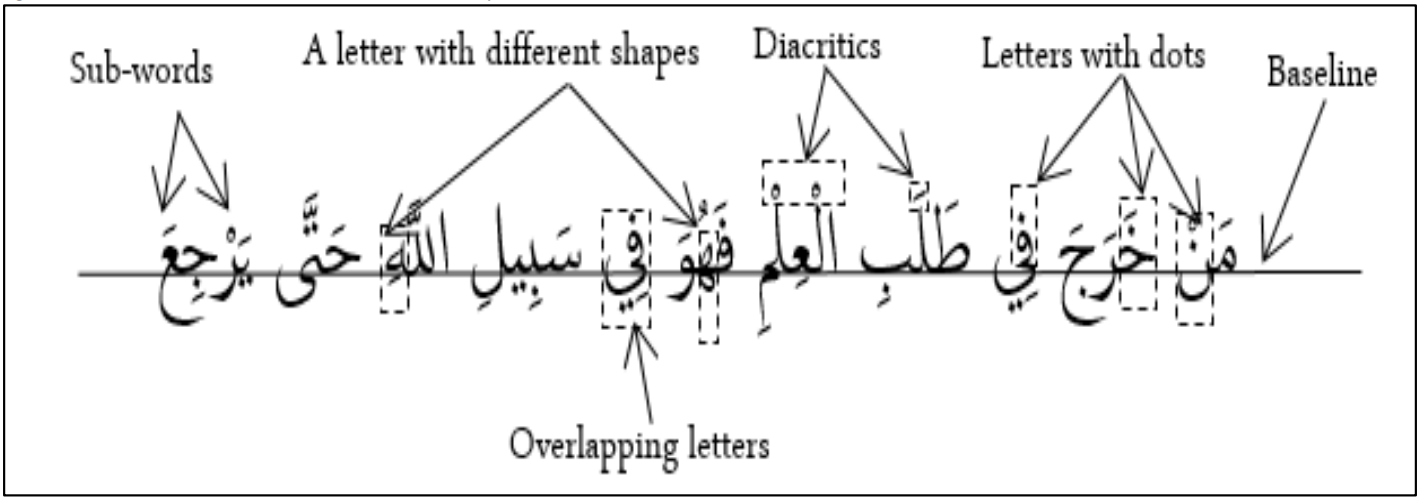
\includegraphics[width=13cm]{images/ocr2.png}
    \caption{Arabic script challenges characteristics.}
    \label{fig:ocr2}
\end{figure}


\textbf{The characteristics of Arabic script that may complicate recognition:}
\begin{itemize}[itemsep=1pt, topsep=5pt]
    \item   Shapes and Positions.
    \item   Overlapping characters and Ligatures
    \item   Diacritics
    \item   Cursive
    \item   Presence of dots
\end{itemize}  

\textbf{GENERAL ARABIC OCR METHODOLOGY (MODEL)}
\begin{figure}[H]
    \centering
    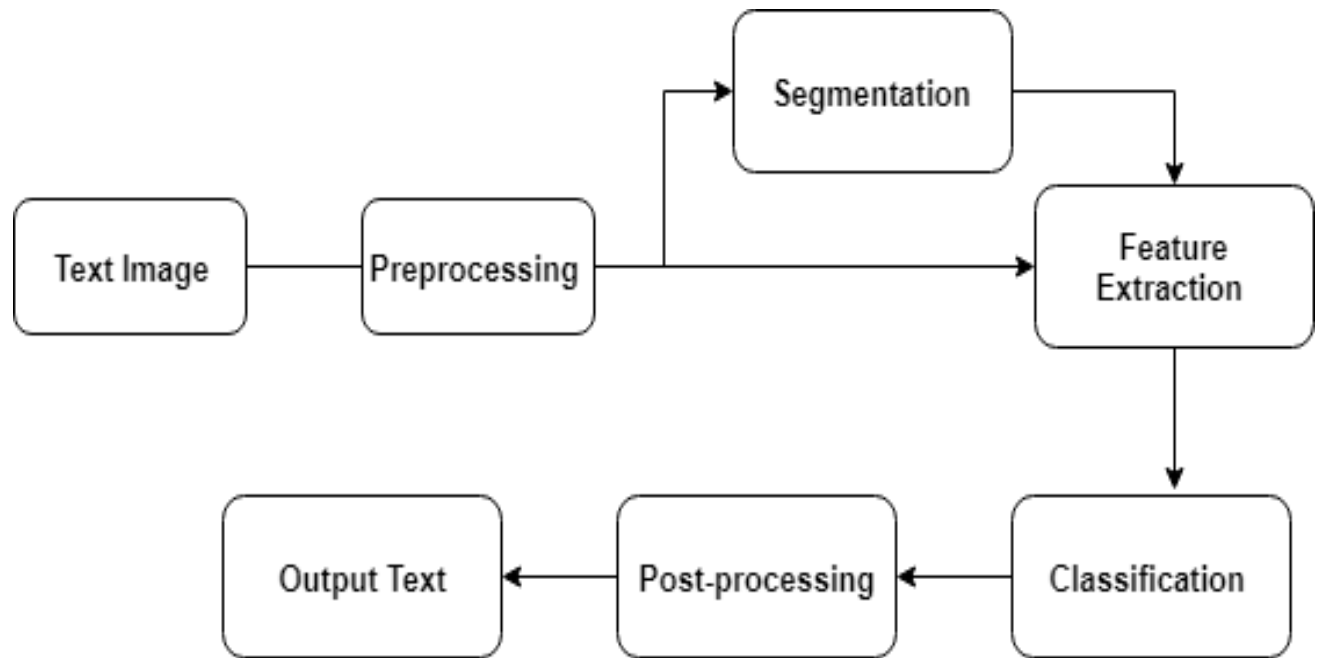
\includegraphics[width=11cm]{images/ocr3.png}
    \caption{General Arabic OCR Methodology}
    \label{fig:ocr3}
\end{figure}

\begin{itemize}[labelindent=1em,labelsep=0.25cm,leftmargin=*]
        \item[\char `A)] \textit{\textbf{Preprocessing:- }} 
        
        This is the first phase of \acrshort{ocr} methodology which is responsible for enhancing the readability of the input image.
Preprocessing is a combination of algorithms that are applied to the input image in order to reduce noise and alterations, thus simplifying the subsequent phases of \acrshort{ocr} methodology. There are various factors that affect the quality of the input image. A study lists the history of images, the printing process, the kind of font, the quality of paper, the condition of the image, and the image acquisition as the vital factors that influence the input image quality. 

Generally, several preprocessing operations are employed on the input image: binarization, layout analysis, thinning, smoothing and filtering, size and slant normalization, slant detection, skew detection, and baseline detection.

However, the selection of these operations, to be applied in the preprocessing, relies upon the conditions of the input image, such as the amount of noise and skew in the input image. 
the preprocessing techniques which are applied in Arabic \acrshort{ocr}:
\begin{itemize}[labelindent=1em,labelsep=0.25cm,leftmargin=*]
        \item[\char `1-] \textit{\textbf{Binarization (thresholding)}} 
        Converting an input grayscale image into a binary image, in which a pixel has only two values 0 and 1
        \item[\char `2-] \textit{\textbf{ Size Normalization}}  
        Size normalization is commonly applied to characters or words by scaling the characters or the words to an adjusted size.
        This process is crucial for the recognition or classification phase.
        
       A study classified normalization methods into two approaches:
       \begin{itemize}[itemsep=1pt, topsep=5pt]
        \item[\char `-]  Moment-based Normalization
        \item[\char `-]  Nonlinear Normalization 
        \end{itemize} 

        \item[\char `3-] \textit{\textbf{De-noising}} 
        
        Noise may have a major impact on the performance of \acrshort{ocr} systems. several techniques have been introduced that are considered noise removal methods:
        \begin{itemize}[itemsep=1pt, topsep=5pt]
        \item[\char `-] Filtering: The median filter approach is commonly used in both printed text images and handwritten text images
        \item[\char `-] Morphological operations (Smoothing)
            \begin{itemize}[itemsep=1pt, topsep=5pt]
            \item Dilation Algorithms, which are applied to broken letters
            \item Erosion Algorithms which are applied to text images with touching letters  
        \end{itemize} 
    \end{itemize} 
       
        \item[\char `4-] \textit{\textbf{Skew Detection and Correction}}
        
        Initially, a text image has zero rotation, yet when physically scanning the image manually, rotation of images up to 20 might occur. This rotation is called skew which results in non-zero skew text images.
        The skew can lead to incorrect recognition and baseline detection.
        It is impossible to segment a text if the text is rotated.
        The process of estimating the skew angle is known as skew detection
        the process of rotating the image with the purpose of correcting the skew is called skew correction
        A wide variety of skew detection and correction methods have been proposed. 
        A study groups these methods into five groups:
        \begin{itemize}[itemsep=1pt, topsep=5pt]
        \item[\char `-] Projection Profile
        \item[\char `-] Hough Transform
        \item[\char `-] Fourier Transform
        \item[\char `-] Nearest Neighbor Clustering 
        \item[\char `-] Correlation
        \end{itemize} 
        \item[\char `5-] \textit{\textbf{Baseline Detection}}
        
        Arabic characters are joined through a horizontal line called the baseline.
        Graphically, the baseline can be described as the line which has the maximal amount of black pixels.
        This line contains critical information about the text, such as text orientation and the position of connection points between Arabic letters.
        The baseline detection techniques for Arabic script have been classified into four groups in :
        \begin{itemize}[itemsep=1pt, topsep=5pt]
            \item[\char `-] Namely
            \item[\char `-] Horizontal projection methods 
             \item[\char `-] Word skeleton method 
            \item[\char `-] Contour tracing and principal component analysis
        \end{itemize} 

         \item[\char `6-] \textit{\textbf{Thinning and Skeletonization}}
         The process of peeling off a pattern as many pixels as possible without affecting the general shape of the pattern In other words, it involves operations that can be implemented in order to produce the skeleton of text images. Thinning is a crucial processing step for text recognition. When applying thinning algorithms to Arabic scripts, various obstacles are encountered. One problem is the reduction in the number of dots in some Arabic characters as a result of the thinning process for which the number of dots is a crucial aspect in differentiating between these characters. Also, dots in Arabic characters are likely to be vulnerable to noise, results are shown in Fig. \ref{fig:thin}

        \textbf{}
        \begin{figure}[H]
            \centering
            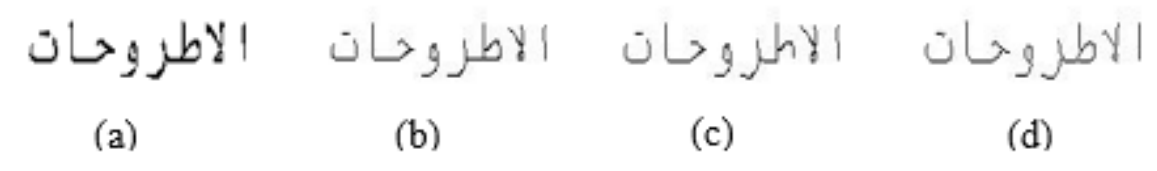
\includegraphics[width=10cm]{images/thin.png}
            \caption{Example results of different thinning algorithms: (a) original word, (b), (c), and (d) thinned word}
            \label{fig:thin}
        \end{figure}
    \end{itemize}

        \item[\char `B)] \textit{\textbf{Line Segmentation:-}}  
        
        During the segmentation phase, the text image is segmented into small components, with a page being segmented into lines, a line into words and a word into letters.
segmenting a text image can be graded into two types: 

\begin{itemize}[itemsep=1pt, topsep=5pt]
    \item External segmentation
    External segmentation refers to the document layout analysis, in particular page decomposition. Generally, it is relatively easy to segment a text line into words in printed text images, compared to handwritten text images which involve overlapping and touching characters by using vertical projection histogram profiles

    \item Internal segmentation
    Internal segmentation deals with segmenting a word into characters. When reviewing segmentation methods in the literature, a major complication arises concerning the classification of word segmentation approaches.

\end{itemize} 

Arabic \acrshort{ocr} systems have been developed by two main paradigms: 
\begin{itemize}[itemsep=1pt, topsep=5pt]
    \item Holistic approaches (segmentation–free) which require a large lexicon of Arabic words.
    \item Analytical approaches (segmentation based) where a word is segmented into units and each unit is recognized separately.
\end{itemize} 

\textbf{}
\begin{figure}[H]
    \centering
    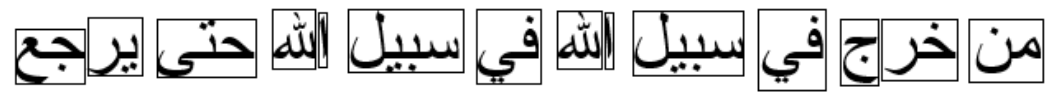
\includegraphics[width=9cm]{images/word.png}
    \caption{Segmenting Arabic lime into its words.}
    \label{fig:word}
\end{figure}

\textbf{}
\begin{figure}[H]
    \centering
    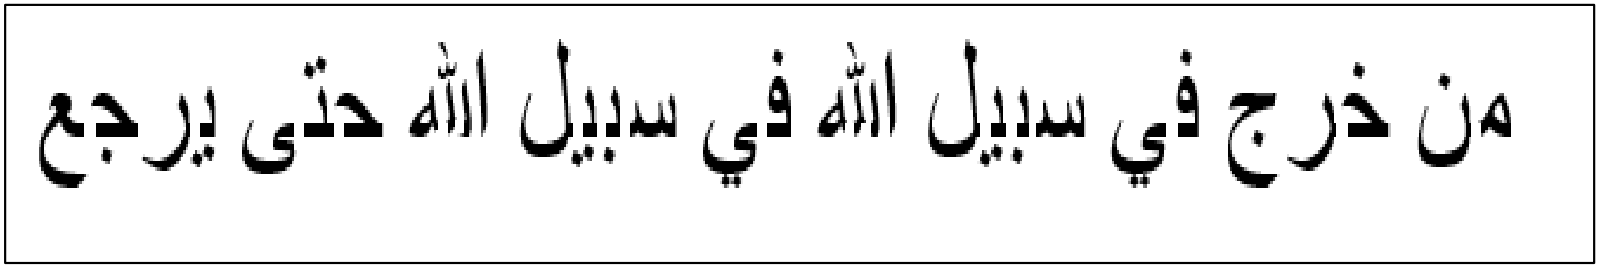
\includegraphics[width=9cm]{images/char.png}
    \caption{Segmenting Arabic words into their characters.}
    \label{fig:char}
\end{figure}

        \item[\char `C)] \textit{\textbf{Feature Extraction:-}} 
        the process of obtaining distinguishing attributes of the segmented character to be utilized by the next phase which is classification. The authors point out that the selection of feature extraction methods depends on the output of the preprocessing stage. The set of features extracted must match the specification of the selected classifier. However, the selection of feature types is a major issue in OCR development.

Such features can be categorized into three groups: 
\begin{itemize}[itemsep=1pt, topsep=5pt]
    \item \textbf{Structural features} which illustrate a text image in terms of its topological and geometrical characteristics by using its local and global properties.

    \item \textbf{Statistical features} which are derived from the statistical representation of patterns that provide a measurable event of interesting patterns. different approaches to produce statistical features. Some examples of the approaches are zoning, moments, characteristic loci, histograms, and crossing.

     \item \textbf{Global Transformation feature} which is applied to convert a skeleton or contour of a pattern by a linear transform into a form that reflects the most relevant features of the transformed pattern.
\end{itemize} 

Finally, the feature extraction stage plays a critical role in Arabic  \acrshort{ocr} development in which distinguishing attributes are extracted and it is clear that each Arabic \acrshort{ocr} developer needs to apply different feature extraction approaches. Still, good features are required, which assist in distinguishing a character from other characters and maximize the accuracy performance simultaneously. Furthermore, these features must be selected specifically for a selected classifier. Some researchers apply different feature extraction methods in combination. However, this may cause extra complications in the implementation.

     
        
        \item[\char `D)] \textit{\textbf{Classification:-}}
        
        The classification phase has the responsibility for assigning a pattern into a pre-classified class based on the features of the pattern which have been extracted in the previous phase. The pre-classified classes can be words, sub-words, characters or strokes, based on the OCR approach used. There are a number of different classification approaches that have been applied for Arabic  \acrshort{ocr}, such as Hidden Markov Models (HMM), Support Vector Machines ( \acrshort{svm}), K-nearest neighbour( \acrshort{knn}).
        
        \item[\char `E)] \textit{\textbf{Post Processing:-}}
        
        Post-processing is the final stage of the development of Arabic \acrshort{ocr}. The objective of this step is to enhance the recognition accuracy by detecting and correcting linguistic misspellings in the produced \acrshort{ocr} text without human intervention Generally, post processing methods can be categorized into two main approaches: lexicon-based methods context-based (statistical) methods.

        The typical technique for correcting the mistakes of Arabic OCR outputs is the lexicon-based method which requires the utilization of an Arabic dictionary. This technique corrects errors without considering any contextual information in which the errors appear.

        \end{itemize}
        \acrshort{ocr} performance evaluation can be classified into two types:
        \begin{itemize}[itemsep=1pt, topsep=5pt]
            \item Black-box evaluation  
            \item White-box evaluation
        \end{itemize} 

        Performance evaluation of \acrshort{ocr} systems is essential for: monitoring the progress of \acrshort{ocr} systems development assessing the effectiveness of \acrshort{ocr} algorithms identifying open areas for further research providing scientific justification for the performance of \acrshort{ocr} systems.\\

For Arabic \acrshort{ocr}, conducting performance evaluation is challenging as no standard dataset is available. This accuracy metric is insufficient to assess how Arabic \acrshort{ocr} systems are overcoming the challenges of Arabic text. However, a study suggests a new set of objective performance metrics for evaluation Arabic \acrshort{ocr} with respect to the challenges of Arabic script which are character accuracy based on character position, dot character accuracy, zigzag-shaped character accuracy, loop-shaped character accuracy, and diacritics accuracy.

\subsection{Convolutional Neural Network(CNN)}
Convolutional Neural Networks (\acrshort{cnn}s) are very effective in perceiving the structure of handwritten characters/words in ways that help in the automatic extraction of distinct features and make \acrshort{cnn} the most suitable approach for solving handwriting recognition problems.\\

This paper \cite{CNN} proposes a method for recognizing the text from manuscript images using Convolutional Neural Networks (CNNs). This includes preprocessing of the manuscript’s image, segmentation of the lines and characters in the manuscript, building a dataset that contains images for each character in different shapes, and classification of each character using CNN.
Fig. \ref{fig:CNN} shows the flow diagram of the proposed methodology.

\begin{figure}[!htb]
    \centering
    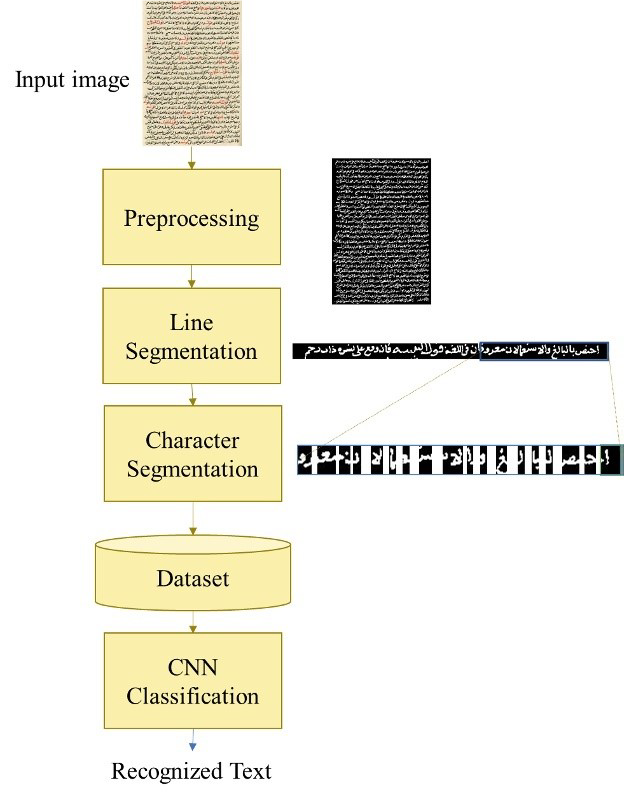
\includegraphics[width=8cm, height=8cm]{images/CNN.png}
    \caption{The flow diagram of the proposed methodology.}
    \label{fig:CNN}
\end{figure}

\begin{itemize}[labelindent=1em,labelsep=0.25cm,leftmargin=*]
        \item[\char `A)] \textit{\textbf{Preprocessing:}} 
        
        The image is transformed into a binary representation.Fig. \ref{fig:pre_cnn} illustrates the preprocessing stages.
        
        \item[\char `B)] \textit{\textbf{Line Segmentation:}}  
        
        Line segmentation is achieved via horizontal Projection Profile (PP) for the image. Horizontal PP is a method used to convert the image from 2D to 1D by calculating the densities \cite{PP}. They used this method to crop out each line at the points of lower density. Fig. \ref{fig:line_cnn} shows the horizontal PP for the whole page, which is used to cut out each line.
        
        \item[\char `C)] \textit{\textbf{Character Segmentation:}} 
        
        Character segmentation is performed using vertical PP. Vertical PP is the same as horizontal PP, but the direction of computing densities is different. In horizontal PP, they calculate the densities for each row. However, in vertical PP the calculation of densities is done for each column. Then, this method is used to cut each character in the line at lower densities of the horizontal PP.Fig. \ref{fig:char_cnn} shows how vertical PP is used to  separate characters of each line in a sentence.
        
        \item[\char `D)] \textit{\textbf{Dataset:}}
        
        They have created three datasets in order to evaluate the classifier. These datasets contain images of Arabic letters in different states.
        
        \begin{enumerate}
        \item {\textbf{First Dataset}}
        
        The first dataset has all 28 Arabic letters with an average of 40 images per letter. The total number of images is 2240 images.
        \item {\textbf{Second Dataset}}
        
        The second dataset has partial letters from the first one. It includes 10 letters. However, we increase the number of images per letter. On average, there are 100 images per letter.
        \item {\textbf{Third Dataset}} 
        
        The third dataset has the same letters presented in the second dataset with an average of 200 images per letter.
        \end{enumerate}
        The data within dataset is randomly divided into a training dataset and validation dataset. 85\% of the data is used for training and 15\% of the data is used for validation. This division is applied to each one of the three created datasets.
        
        
        \begin{figure}[!htb]
        \centering
        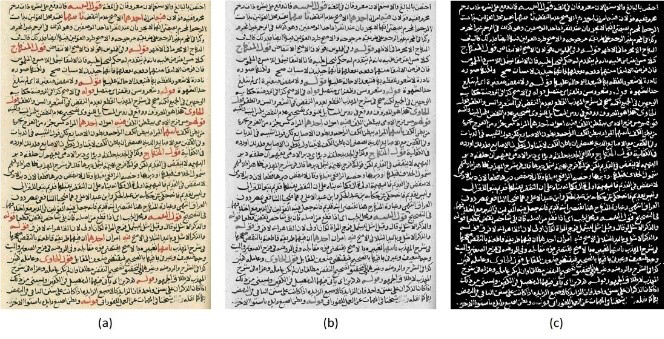
\includegraphics[width=10cm]{images/pre_cnn.png}
        \caption{(a) Original image. (b) Grayscale image. (c) Binary image.}
        \label{fig:pre_cnn}
        \end{figure}
        
        \begin{figure}[!htb]
        \centering
        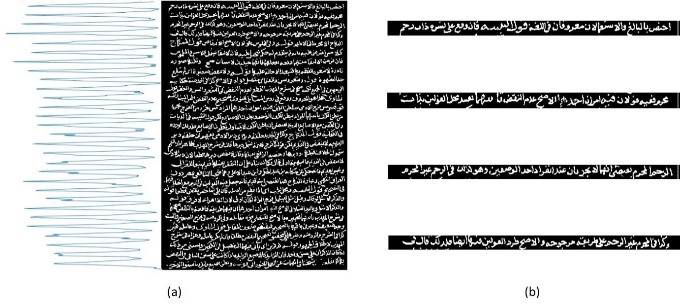
\includegraphics[width=10cm]{images/line_cnn.png}
        \caption{(a) Horizontal Projection Profile for the whole page image. (b) The segmentation of the first four lines.}
        \label{fig:line_cnn}
        \end{figure}
        
        \begin{figure}[!htb]
        \centering
        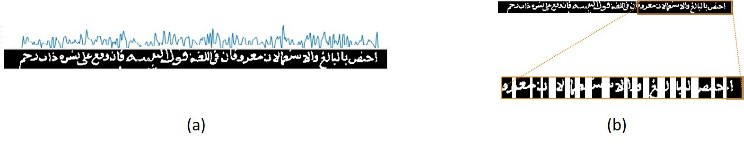
\includegraphics[width=10cm]{images/char_cnn.png}
        \caption{(a) : Vertical PP for a line. (b) : Character segmentation for the first characters in the line.}
        \label{fig:char_cnn}
        \end{figure}
        
        
        \item[\char `E)] \textit{\textbf{\acrshort{cnn} Classification:}}
        
        Convolutional Neural Networks (\acrshort{cnn}s) are feedforward networks. In particular, the data flows within CNN in one direction only. In general, CNN consists of one or more convolutional and pooling layers followed by one or more fully connected layers. Fig. \ref{fig:cnn_leyar} shows the general CNN architecture for an image classification task.
        
        they defined the \acrshort{cnn} architecture for Arabic characters images classification as follow:
        \begin{enumerate}
        \item {\textbf{Input Layer:}}
       The input is an image that represents a single character from the historical Arabic manuscripts. We specify the image size to be 30-by-30-by-1 for all input images. The height and the width for the input image is equal to 30 pixels. As our images are grayscale images, the channel size is 1. images.
       
        \item {\textbf{Convolutional Layers:}}
        The convolution operation is a mathematical The convolution operation is a mathematical operation that takes an image along with a filter of a specific dimension, mostly an odd number, and applies this filter along with the image. An example of convolution is shown in figure \ref{fig:cnn-onvolution}. \\
        
        three convolutional layers. Each layer is followed by a
        nonlinear activation function, which is ReLU. The number of neurons varies in each convolutional layer. Particularly, the first layer has 8 neurons, the second layer has 16 neurons, and the third layer has 32 neurons.
        
        \begin{figure}[!htb]
        \centering
        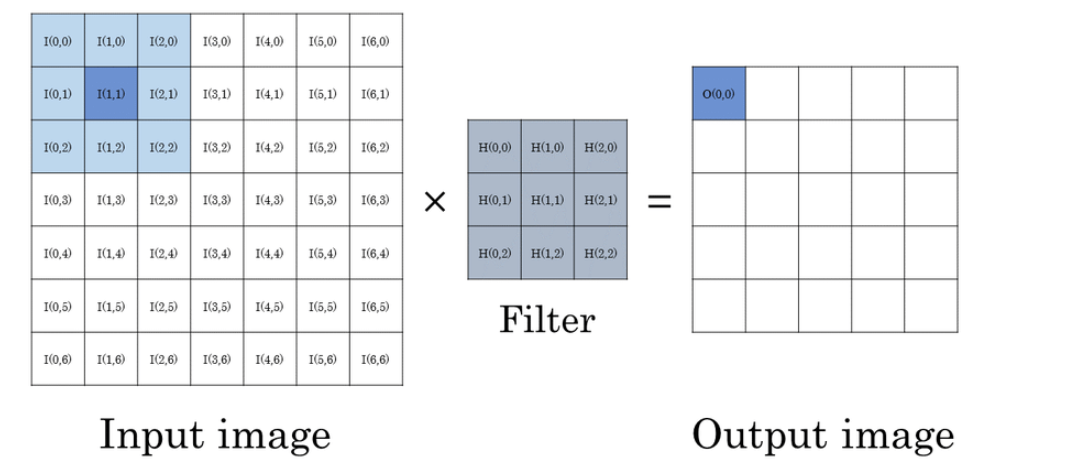
\includegraphics[width=8cm]{images/cnn-convolution.png}
        \caption{Example for convolution operation with the filter of size 3x3}
        \label{fig:cnn-onvolution}
        \end{figure}
        
        \item {\textbf{Max Pooling Layers:}} 
Each convolutional layer is
followed by a down-sampling operation that reduces the
spatial resolution of the feature map. One way of downsampling
is to use max pooling, which returns the maximum
values of rectangular fields of inputs. The two arguments that
specify max pooling operation are pool size and step size.
Pool size is the size of the rectangular field of the input. Step
size specifies the size that the training function takes as it
scans along with the input. they made both pool size and step size
to equal 2.

        \item {\textbf{Fully Connected Layer:}} 
In this layer, the neurons
connect to all neurons in the previous layer in order to
combine all features learned by the previous layers to identify
class label. Therefore, the number of neurons in this layer is
equal to the number of classes in the target dataset.

        \item {\textbf{Output Layer:}} 
This layer uses the probabilities
returned by the Softmax activation function for each input
and assign the input to one of the output classes.
        \end{enumerate}
        
        \begin{figure}[!htb]
        \centering
        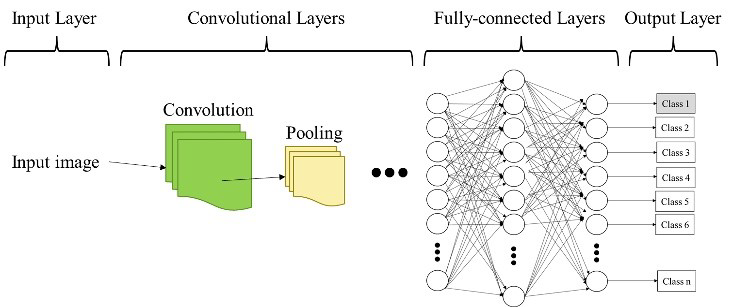
\includegraphics[width=10cm]{images/cnn_leyar.png}
        \caption{The general CNN architecture for an image classification task.}
        \label{fig:cnn_leyar}
        \end{figure}
        
    \end{itemize}
They applied \acrshort{cnn} classification to the three datasets and
compute the accuracy resulting from applying CNN on each
dataset. Dataset1, which contains 56 classes with 40 images
per class, gives an accuracy of 74.29\%. On the other hand,
Dataset2 and Dataset3 give higher accuracies: 84.67\% and
88.20\%, respectively.

\section{Datasets}
Finding the appropriate and balanced data on which to work on and train the model is critical to the success of the experiments that take place during the work, so it was necessary to find a dataset that has a high degree of accuracy and also a large number of words that the model trains on. The stage of searching for a suitable dataset was very difficult so we decided to study all the available datasets that we found during the survey process. \\

Here, we review some of the datasets that we have studied, show the advantages and disadvantages of each, choose the most suitable dataset for us and mention its features in detail.

\subsection{Arabic Handwritten Character Dataset (AHCD)}
An open-source database of 16,800 characters was written by 60 participants; Their ages range from 19 to 40 years. It was used in more than one scientific paper concerned with recognizing handwritten Arabic words so that the accuracy of working with the \acrshort{cnn} model reached 97\% sometimes.\cite{altwaijry2021arabic} It is characterized by the diversity of fonts in it, but it was not suitable for the work we want because it is included in the intelligent systems that are interested in recognizing the handwritten Arabic language using the pen and modern writing tools. 

Not suitable because the way we decided to work on this project depends mainly on words and not characters. Fig\ref{fig:AHCD sample}

\begin{figure}[!htb]
    \centering
    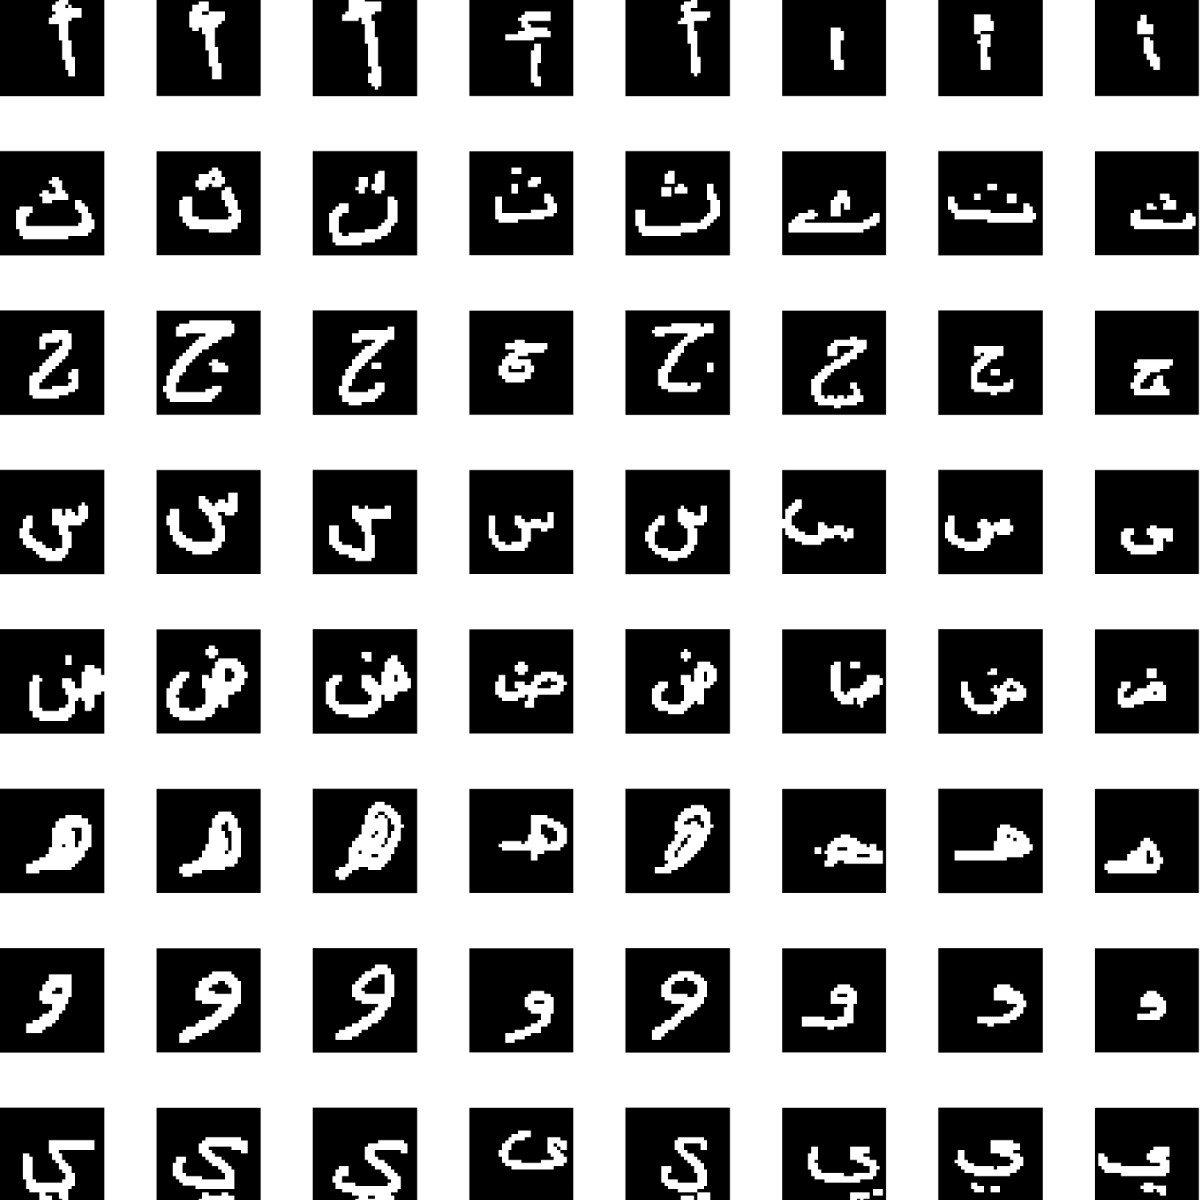
\includegraphics[width=7cm]{images/AHCD sample.png}
    \caption{Example from the AHCD dataset}
    \label{fig:AHCD sample}
\end{figure}

\subsection{Hijjaa Dataset}
The open-source database is written exclusively by children between the ages of 7 and 12. This dataset contains 47,434 characters written by 591 participants. It was used in one scientific paper we saw during the survey phase on the recognition of handwritten Arabic words until the accuracy of working with the \acrshort{cnn} model reached 88\%.\cite{altwaijry2021arabic} But it is also written with modern tools such as the pen and was written by the hands of young children and is also divided into letters, and as we mentioned it does not fit the method of work we have chosen. You can download the dataset from \url{https://github.com/israksu/Hijja2}

\subsection{KHATT Dataset}
KHATT dataset \cite{KHATT} is a constructed dataset consisting of images containing Arabic text collected from the web along with their ground truth.
A portion of the text includes Arabic diacritics. and Multiple Arabic fonts that closely resemble the old fonts used in historical manuscripts (dating back to the 18th century) are used. We show an example in Fig\ref{fig:Sample-text-images-from-the-KHATT-dataset}

There are four categories of images:

\begin{itemize}[itemsep=1pt, topsep=5pt]
    \item Full sequences (i.e., images with more than five words).
    \item Short sequences (i.e., images that have five or fewer words), Full sequences.
    \item With diacritics (the images with more than five words with diacritics).
    \item Short sequences with diacritics (images with five or fewer words, with diacritics).
\end{itemize}  

The handwritten manuscripts from the KHATT database are also included (KHATT contains unconstrained handwritten Arabic Texts written by 1000 different writers).\cite{mostafa2021ocformer}

\begin{figure}[!htb]
    \centering
    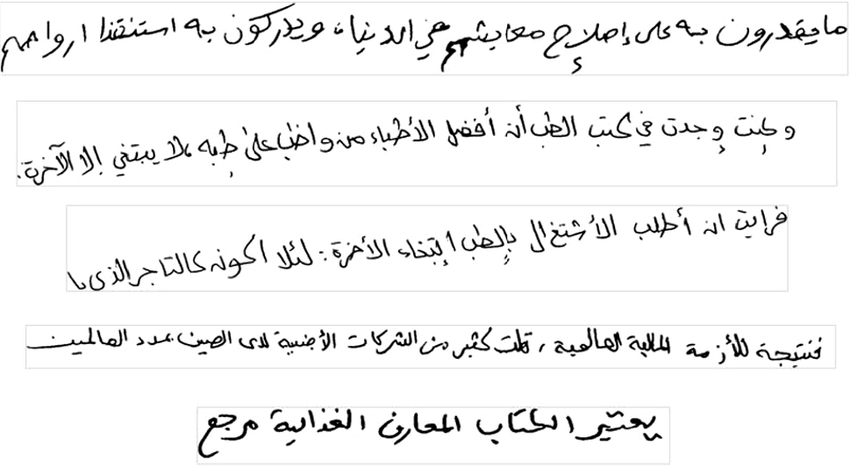
\includegraphics[width=10cm]{images/Sample-text-images-from-the-KHATT-database.PNG}
    \caption{Example from the KHATT dataset}
    \label{fig:Sample-text-images-from-the-KHATT-dataset}
\end{figure}


\subsection{IFN/ENIT Dataset}
The IFN/ENIT \cite{IFNENIT} database contains training and testing materials for Arabic handwriting recognition software. There are more than 2,200 binary images of sample figures in handwriting from 411 writers\cite{ali2019efficient}, but they are not suitable for work in manuscripts due to the different tools of the book and are not similar to the nature of Arabic manuscripts and their number is also very small in relation to other datasets. We show an example of them in the fig\ref{fig:Sample text images from the IFN/ENIT dataset}

\begin{figure}[!htb]
    \centering
    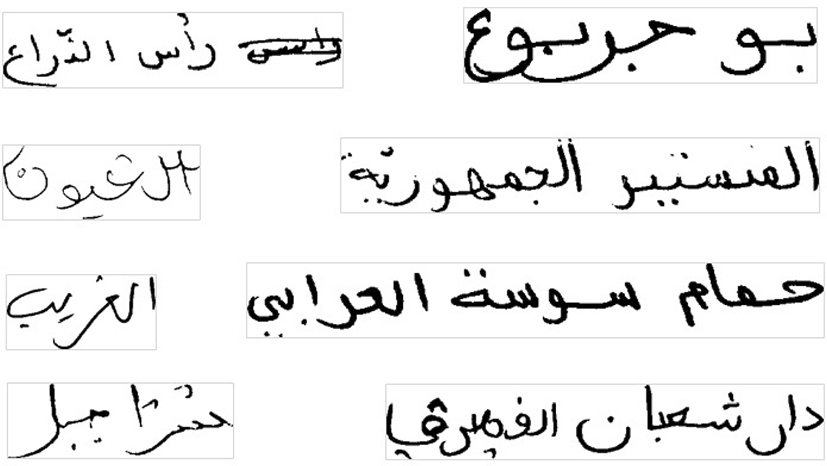
\includegraphics[width=8cm]{images/Sample-text-images-from-the-IFN-ENIT-database.png}
    \caption{Sample text images from the IFN/ENIT dataset}
    \label{fig:Sample text images from the IFN/ENIT dataset}
\end{figure}

\subsection{RASAM (Maghrebi) Dataset}
In the paper \cite{RASAM} present a Maghrebi dataset, This Dataset is made up of 300 annotated images, with their related ground truth stored in an XML file (page XML format). Images come from three manuscripts selected among the collections of the Bibliotheque Universitaires des LAngues et Civilisations (BULAC): two manuscripts belong to the historical genre (MS.ARA.1977 and MS.AR.417) and the third one has to do with inheritance law (MS.ARA.609). An example of RASAM dataset is shown in the figure \ref{fig:RASAM sample dataset}

The images of the dataset are in JPEG format and have varying resolutions from 96 DPI to 400 DPI.

\begin{figure}[!htb]
    \centering
    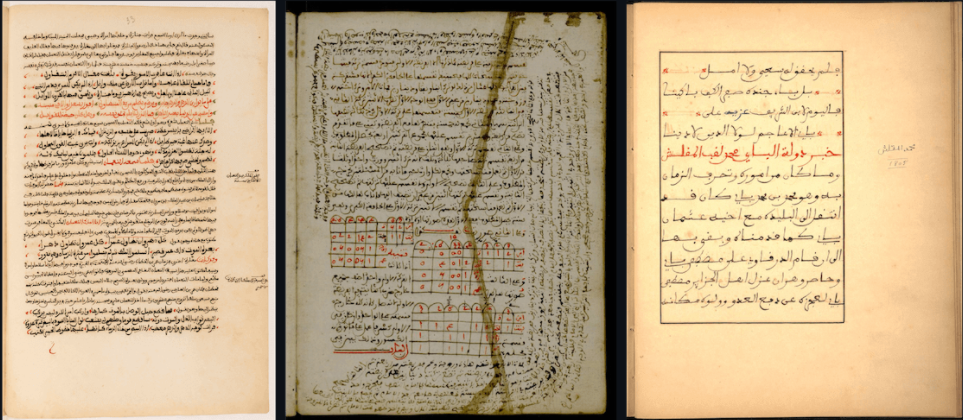
\includegraphics[width=10cm , height=7cm]{images/RASAM sample.png}
    \caption{Sample text images from the RASAM dataset}
    \label{fig:RASAM sample dataset}
\end{figure}

\subsection{IBN SINA Dataset}
It is a dataset that has been published and is taken from a philosophical book by Ibn Sina, Allows images in binary and color formats, The dataset consists of 51 folios which correspond to 20722 CCs (almost 500 CC on each folio)\cite{farrahi2010ibn}.
This dataset has been used in many scientific papers that we have seen in the survey phase and has had very good results, especially when it is used in a CNN-GRU model\cite{hassen2021subword}.
This set of data has many features such as it is large in proportion to the training of the model, and also the images are in color and gray, but they are from one book and in one font and indicate the shape of the letters in a specific time period, and it does not have the diversity required in our project to identify the largest number of manuscripts.

\begin{figure}[!htb]
    \centering
    \begin{minipage}{0.45\linewidth}
        \centering
        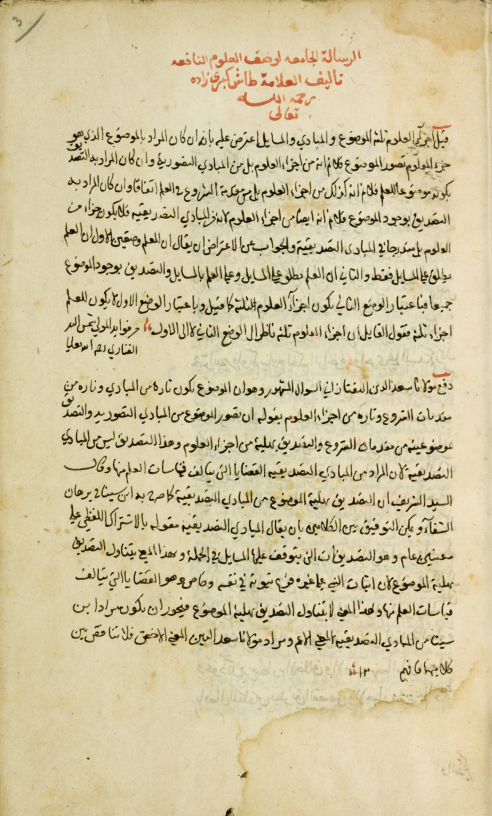
\includegraphics[width=0.7\linewidth, height=0.9\linewidth]{images/IBN SINA original image.png} % first figure itself
        \caption{Sample of the original image in IBN SINA dataset}
        \label{fig:adaptive-gaussian}
    \end{minipage}\hfill
    \begin{minipage}{0.45\linewidth}
        \centering
        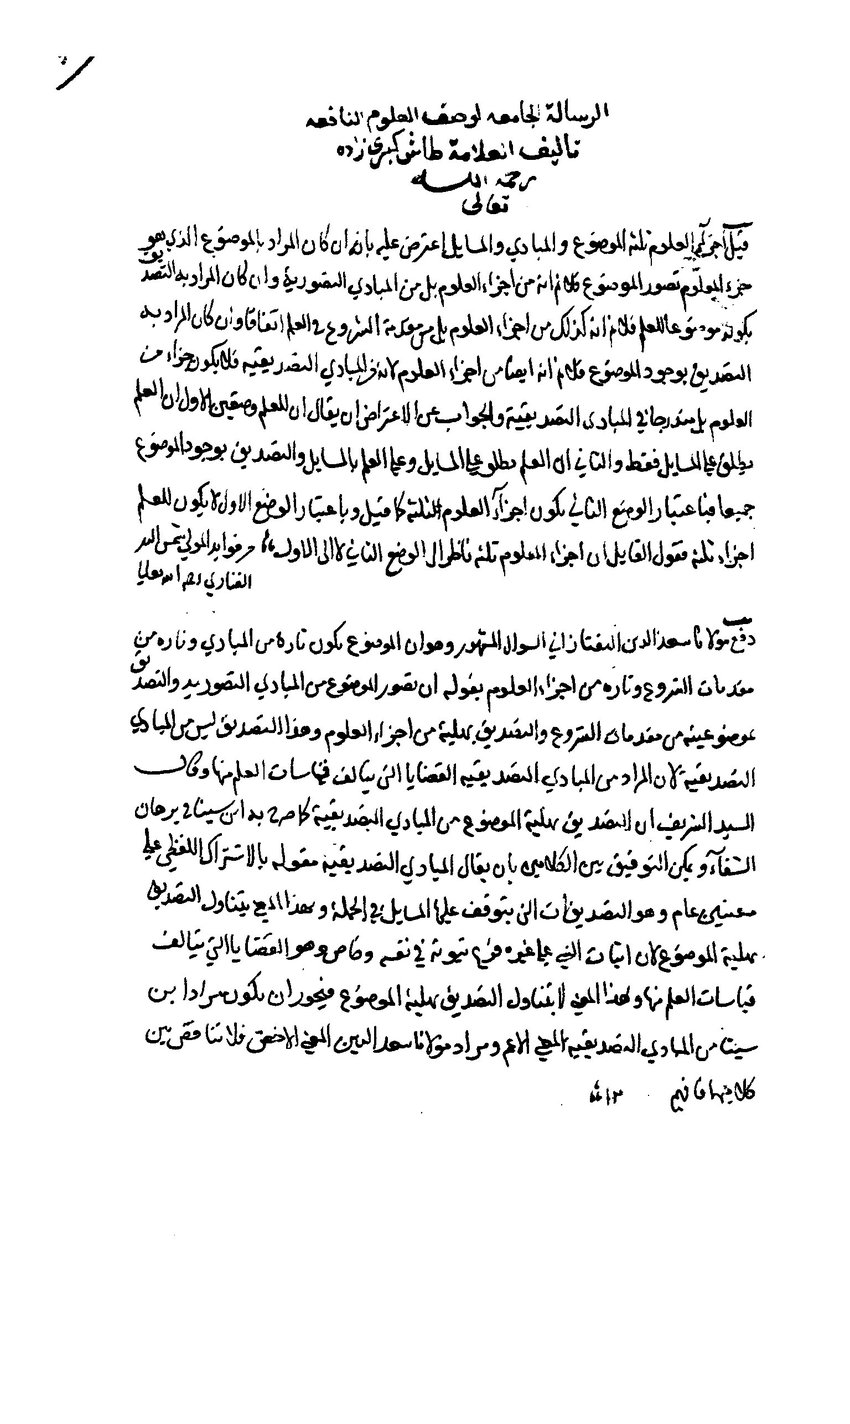
\includegraphics[width=0.7\linewidth, height=0.9\linewidth]{images/IBN_SINA binarized sample.png} % second figure itself
        \caption{Sample of the binarized image in IBN SINA dataset}
        \label{fig:IBN_SINA binarized sample}
    \end{minipage}
\end{figure}


\subsection{VML-HD Dataset}
In the paper \cite{VMLHD} present a new database with a handwritten Arabic script. This dataset is based on five books written by different authors in the years 1088 - 1451 fig\ref{fig:VML-HD sample dataset}, and the entire 668 pages are annotated at the sub-word level. For each page, we manually applied bounding boxes to the different subwords and annotated the character sequences. It consists of 159,149 subwords of 326,289 letters of a vocabulary of 5509 forms of subwords. \\
One of the advantages of this data set is that it contains examples of 5 books of different formats and character shapes, and they indicate five different eras in Arab Islamic history.

\begin{figure}[!htb]
    \centering
    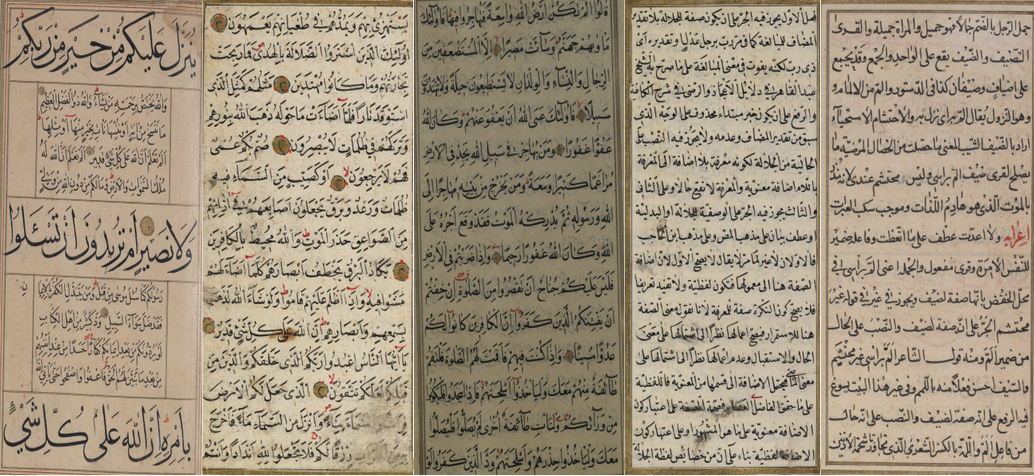
\includegraphics[width=15cm]{images/vml-hd-sample.PNG}
    \caption{Sample text images from the five books that make up the VML-HD dataset}
    \label{fig:VML-HD sample dataset}
\end{figure}

It was created by a team from one of the universities in the Middle East and they made a great effort, they used in this work a WebGT ground truth system\cite{biller2013webgt}, which is a web-based system for ground truth generation and provides a user-friendly interface for quick annotation of degraded documents in general, and historical document images in particular. Using this system they marked the bounding of the sub-words found on each page. They manually applied each bounding box around the sub-words present in the image, then they annotated each bounding box with its corresponding sequence of characters. they have marked, in total, 121,636 sub-words of 1,731 different forms of sub-words.\cite{VMLHD}


\begin{figure}[!htb]
    \centering
    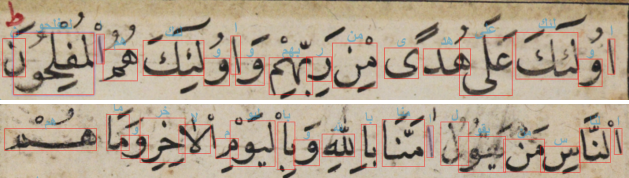
\includegraphics[width=10cm, height=3cm]{images/Web-GT.png}
    \caption{An example of an annotated line done using Web-GT framework.}
    \label{fig:Web-GT.png}
\end{figure}

The WebGT website exports an XML file in Hadara\cite{pantke2013hadara} format. Each book has its own Hadara XML file which contains the coordinates of all the bounding boxes of all the images annotated in that book, as well as the sequence of characters for each bounding box applied in Arabic text. They also generated a Hadara XML file for each page in addition to the file for each book. This file contains the coordinates of the bounding boxes and the sequence of the characters for the specific page only. Finally, to alleviate any encoding issues, they also released encoded files of the same format. These files have for each letter written in Arabic script a corresponding Latin symbol that will denote such a letter. \\

Finally, they generated the ground truth data for each sub-word found in the dataset. The ground truth data consists of the following fields: Book number, Page number, Sub-word id, Location coordinates, Arabic annotation, Latin annotation, and Sub-word length. Two examples of the ground truth gathered for sub-words can be seen in Table \ref{table:2.1}.

\begin{table}[!htb]
\begin{center}
\begin{tabular}[htbp!]{ | c | m{3cm}| m{3cm} | } 
  \hline
  Image & 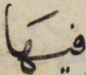
\includegraphics[width=1.5cm ]{images/feha.png} & 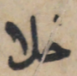
\includegraphics[width=1.5cm ]{images/khla.png} \\ 
  \hline
  Book number & 3158466 & 187370 \\ 
  \hline
  Page number & 006-2 & 0013-2 \\ 
  \hline
  Segment id & 183380 & 187370 \\ 
  \hline
  Location coordinates & y=1249 x=856  y=1249 x=945  y=1352 x=945
 y=1352   x=856 & y=1212 x=649  y=1212 x=722  y=1306 x=722  y=1306  x=649 \\ 
   \hline
  Arabic annotation & \<فيها>\ &\<خلا> \\ 
  \hline
\end{tabular}
\end{center}
\caption{Two examples of ground truth information for each sub-word in the VML-HD dataset.}
\label{table:2.1}
\end{table}

\section{Image Preprocessing}
In this section, we will be discussing our experiments performing preprocessing on images shown in Fig.\ref{fig:preprocessing} . we have used Python language, Which includes using different libraries. The main ones are OpenCV and scikit-image.

\begin{figure}[!htb]
    \centering
    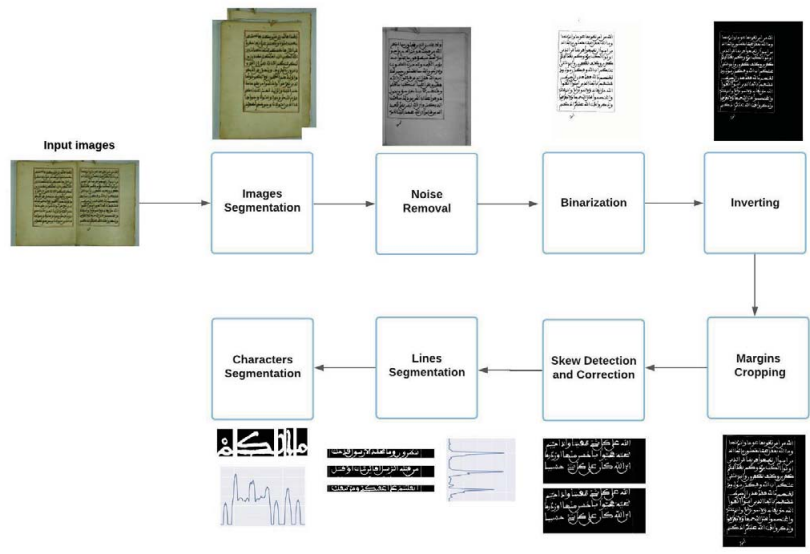
\includegraphics[width=14cm]{images/preprocessing.png}
    \caption{Preprocessing steps for segmentation}
    \label{fig:preprocessing}
\end{figure}

\begin{itemize}[labelindent=1em,labelsep=0.25cm,leftmargin=*]
        \item[\char `A)] \textit{\textbf{Noise Removal:-}} 
       
        In paper, \cite{Shams2020} This step focuses on removing any noise from the images
        which contain the text to be segmented. 
        Since the manuscript is ancient and written more than 250
        years ago, pages contain a considerable amount of noise.
        Furthermore, an important characteristic of the Arabic language is
        diacritics which can be added to letters in different locations,
        e.g., at the top or the bottom of the letter. These diacritics make
        the text segmentation process more complicated. As a solution
        to this, colored images of the manuscripts were split into three
        main channels: R, G, and B. After that, the R channel was
        chosen as it was the clearest one among them.
        Another step of noise removal that was taken is applying
        Gaussian filter is in charge of smoothing the image.
        \item[\char `B)] \textit{\textbf{Binarization and Inverting:-}}
        
        This step aims to convert the colored images into binary
        images where the text (foreground) is in white and the background is in black. This is required in the PP method.
        Firstly, the images are converted into grayscale. Secondly,
        images are converted into binary by applying a specific
        thresholding technique. For this reason, different methods were
        applied to a sample of the manuscript in order to achieve the
        best results. There are two main types of thresholding methods: global and local. Global methods choose one threshold value for the whole image. On the other hand, local methods choose
        a different threshold value for each pixel by calculating the
        features of its neighbors. Firstly, two local methods were
        applied which are adaptive Gaussian thresholding in 
        Fig. \ref{fig:adaptive-gaussian} and adaptive mean thresholding in Fig. \ref{fig:adaptive-mean} 
        
        \begin{figure}[!htb]
            \centering
            \begin{minipage}{0.45\linewidth}
                \centering
                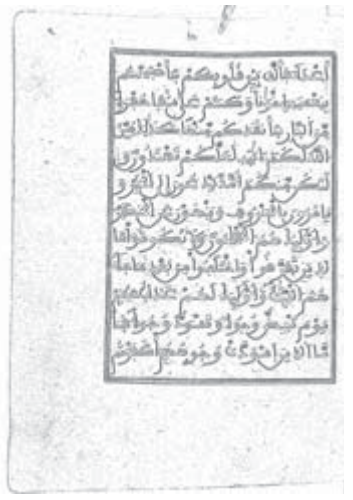
\includegraphics[width=0.7\linewidth, height=0.9\linewidth]{images/adaptive-gaussian.png} % first figure itself
                \caption{Adaptive Gaussian}
                \label{fig:adaptive-gaussian}
            \end{minipage}\hfill
            \begin{minipage}{0.45\linewidth}
                \centering
                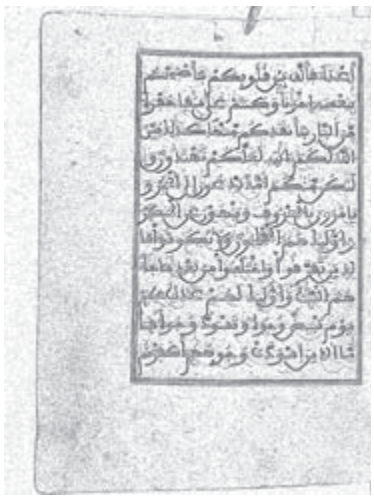
\includegraphics[width=0.7\linewidth, height=0.9\linewidth]{images/adaptive-mean.png} % second figure itself
                \caption{Adaptive Mean}
                \label{fig:adaptive-mean}
            \end{minipage}
        \end{figure}
        
        It is clear that both results are considered poor. So, other global methods were applied such as mean in Fig. \ref{fig:thresholding} a, Otsu in Fig. \ref{fig:thresholding} b, and
        minimum in Fig. \ref{fig:thresholding} c. It is clear that the minimum method gives out
        the best result so it was the chosen method for binarization.
        
        \begin{figure}[!htb]
            \centering
            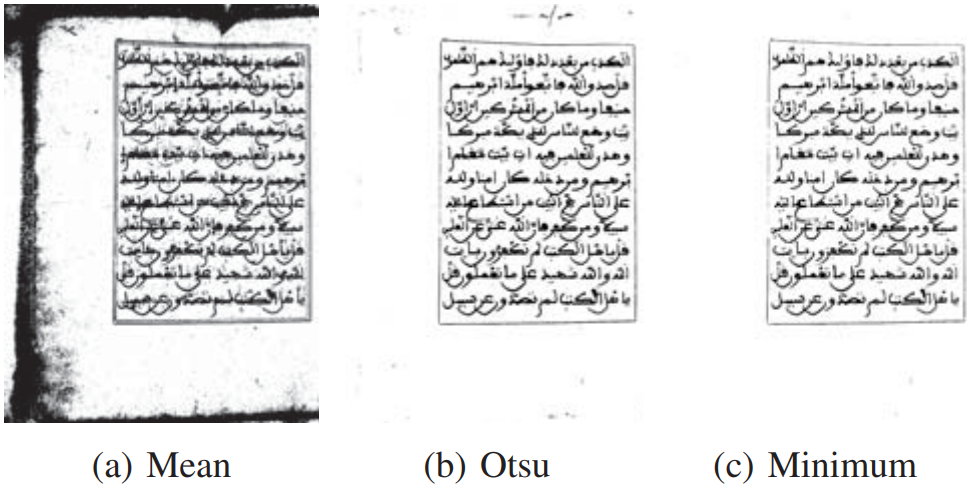
\includegraphics[width=10cm]{images/thresholding.png}
            \caption{Global thresholding methods results}
            \label{fig:thresholding}
        \end{figure}
        
        After applying the binarization, the result was the text
        (foreground) in black color and the background in white color.
        In order to make the text become more clear, the inverting step
        was performed where the text (foreground) has become in
        white color and the background in black color.
        
        \item[\char `C)] \textit{\textbf{Margins Cropping:-}} 
        
        Each page in the original manuscript contains margins in
        three directions depending on the side of the written text.
        Therefore, it was needed to crop these margins so that the
        images will contain only text without empty spaces.
        This process is composed of many steps. Firstly, inverted
        images are used as input, then the adaptive (local) threshold is
        calculated for each block, where the block size is set to 35 and
        the max value of the threshold is set to 255. After that, erosion
        method is applied to the image using a structural element of
        size 40×40. Then, a mask is extracted from the erosion image
        by applying a global thresholding with a value of 120. The next
        step is that the edges of the images are detected and the max and min values of both x and y axes are calculated. Finally,
        these values will be used to crop image’s margins.
       
        \item[\char `D)] \textit{\textbf{Skew Detection and Correction:-}}
        
        Skew happens when the image is not set correctly on the
        scanner or the camera, which results in poor accuracy in the
        segmentation phase.
        Some parts of the manuscript contain skewed images which
        will therefore affect the segmentation phase. Therefore, a skew
        detection and correction method was applied where the binary
        image is used as input. Then, different values of angles are
        tested in order to find the best angle value. This is done by
        calculating the Horizontal PP. The difference between each
        value and the value next to it powered by two is calculated. If
        the image is skewed, the sum of the differences between these
        two values will be small. In contrast, if the image’s skew is
        set correctly, the difference between them will be large. To
        clarify this further, Fig. \ref{fig:skew} shows two Horizontal PP, where
        Fig. \ref{fig:skew}a is the correctly skewed page, and Fig. \ref{fig:skew}b is the same
        page but after rotating it by 30°. Finally, the angle that leads
        to the maximum score will be chosen. After that, the image
        will be rotated using this angle value.
        \begin{figure}[!htb]
            \centering
            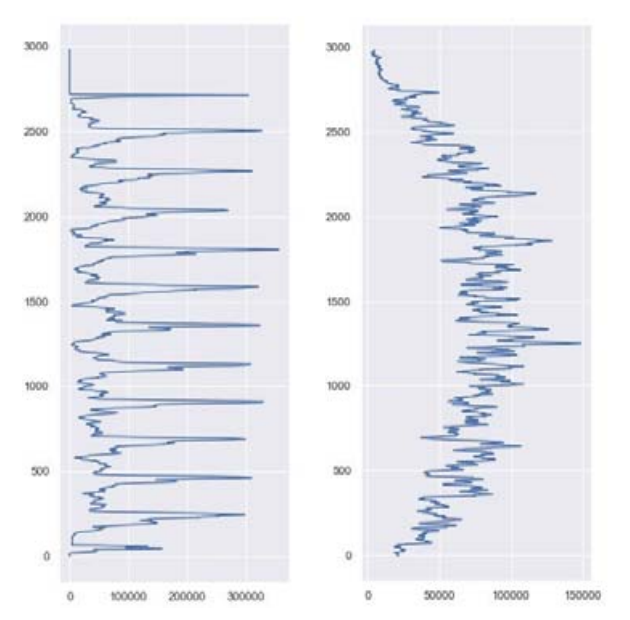
\includegraphics[width=7cm]{images/skew.png}
            \caption{The effect of skew on Horizontal PP}
            \label{fig:skew}
        \end{figure}
    \end{itemize}

\section{Line Segmentation}
Text-lines are hard to segment in the context of Arabic manuscripts, because of the narrowly spaced text lines with touching or overlapping components, the varying spaces between words, the ascendant or descendant letters, special marks, and dots, calligraphy, etc.\\

In this paper \cite{9257759} the
the proposed system is used  to automatically extract text lines from images of unconstrained handwritten Arabic texts. Each text line is detected by its baseline based on text-line masks which are predicted by a deep neural network called \acrshort{AR2U} based on the U-Net model with an Attention mechanism. The \acrshort{AR2U} model is used to allow a pixel-wise classification and therefore to separate text-lines pixels from the background one.
It tested on BADAM: a Public Dataset for
Baseline Detection in Arabic script Manuscripts that involves complex layouts as well as curved and arbitrarily oriented text-lines and overlaps between adjacent text-lines, words, or sub-words  Fig \ref{fig:example1}.\\ 

This model achieves the best performance with a Precision of 0.932\% which competes with current state-of-theart approaches.Fig \ref{fig:example2} shows an example of model prediction on an image
of the dataset.

\begin{figure}
    \centering
    \begin{minipage}{0.45\linewidth}
        \centering
        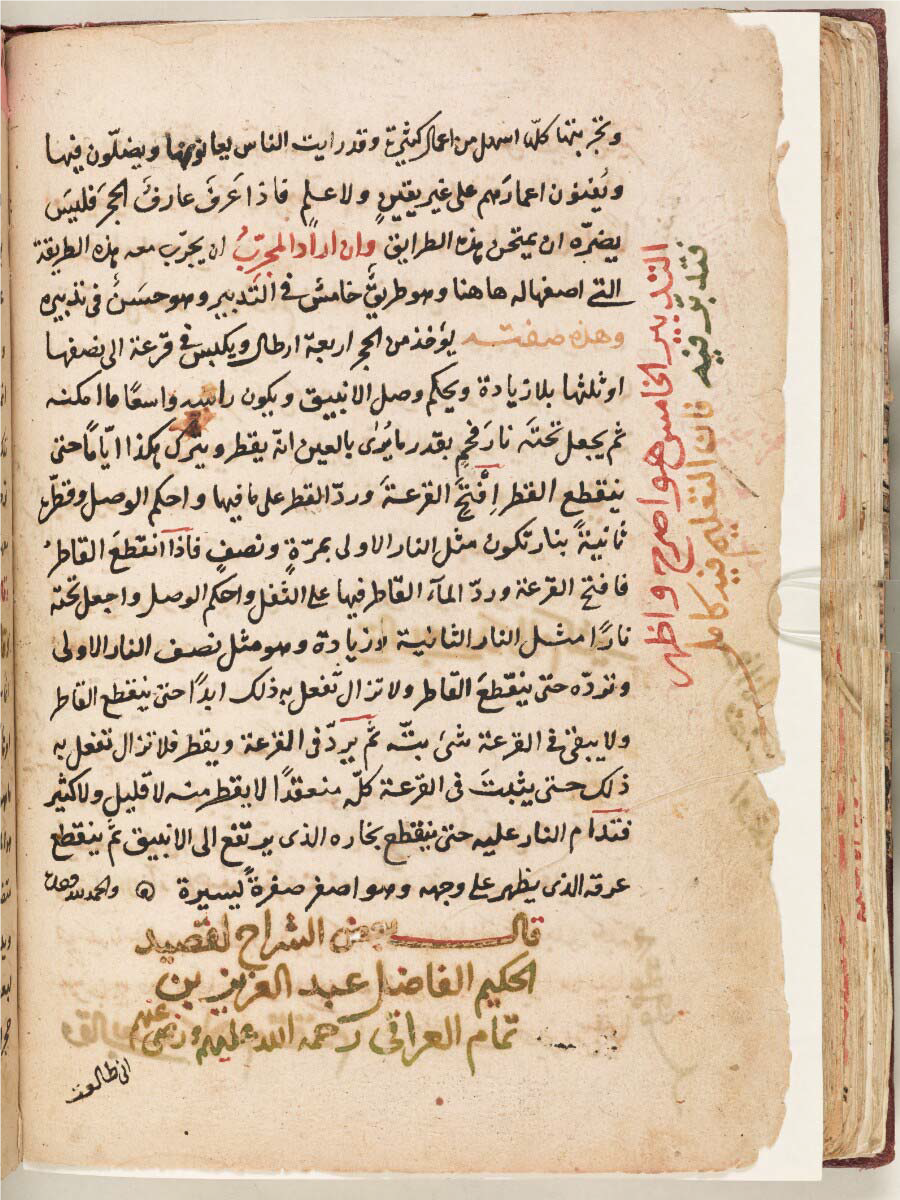
\includegraphics[width=0.7\linewidth, height=0.9\linewidth]{images/example.png} % first figure itself
        \caption{Example of used documents.}
        \label{fig:example1}
    \end{minipage}\hfill
    \begin{minipage}{0.45\linewidth}
        \centering
        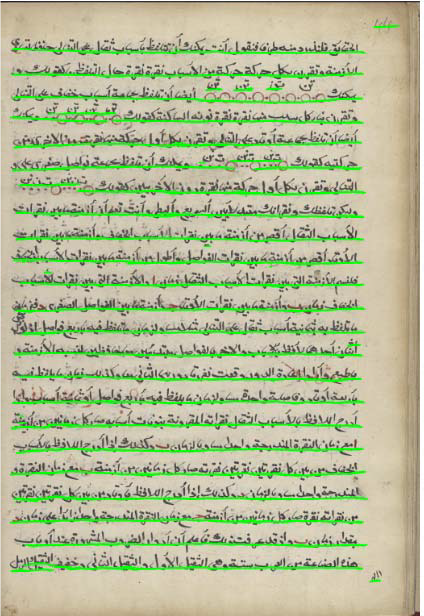
\includegraphics[width=0.7\linewidth, height=0.9\linewidth]{images/example2.png} % second figure itself
        \caption{Example of model predictions result.}
        \label{fig:example2}
    \end{minipage}
\end{figure}

This paper \cite{8892920} proposed a novel approach to carry out the segmentation of Arabic manuscripts into text-lines and words, using deep learning. The proposed text-line segmentation system uses an \acrshort{RU} to extract x-heights from text images, then a post-processing step extracts baselines Fig \ref{fig:X-height}. The word segmentation system uses a \acrshort{cnn} with a \acrshort{blstm}, then a \acrshort{ctc} to find the alignment between the text-line transcription and the text-line image.

\begin{figure}[!htb]
    \centering
    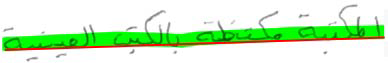
\includegraphics[width=10cm]{images/X-height.png}
    \caption{X-height (green) and baseline (red) of a text line.}
    \label{fig:X-height}
\end{figure}

\begin{itemize}[labelindent=1em,labelsep=0.25cm,leftmargin=*]
         \item[\char `A)] \textit{\textbf{Text-line Segmentation}} 
         
        For text-line segmentation, we extracted the x-heights of
        text-lines, by the use of a ground truth that separates the input images into three classes:
        \begin{enumerate}
            \item Background.
            \item Paragraphs.
            \item Text-lines x-heights in each paragraph.
        \end{enumerate}
        as shown in Fig \ref{fig:result_of_line}(b).
        
        \begin{figure}[!htb]
            \centering
            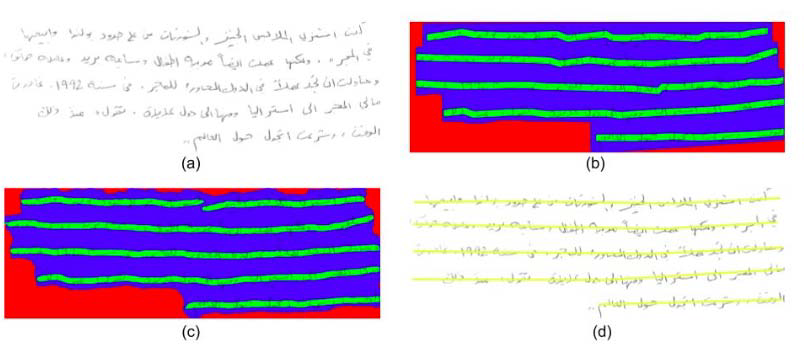
\includegraphics[width=9cm]{images/result_of_line.png}
            \caption{Results of text-line segmentation: a) the original image, b) the ground truth composed of three classes (background: red; paragraph: blue; x-height: green), c) the output of the RU-net, d) the final result after post-processing.}
            \label{fig:result_of_line}
        \end{figure}
        
        \item[\char `B)] \textit{\textbf{Word Segmentation}}
        
        For word segmentation, firstly used a \acrshort{cnn} to extract the most important features from the text-line images. All images have a normalized size of 48×1600. Every convolutional block is followed by a batch normalization that greatly reduces the vanishing gradient problem and makes the use of dropout unnecessary. The output of the \acrshort{cnn} is then sequentially passed to a \acrshort{blstm} having 100 neurons for each LSTM and followed by a \acrshort{ctc} function, as shown in Fig \ref{fig:seg_network}
        
        Their two classes: \textbf{word}(1) and \textbf{space}(2). The
        provided ground truth is the text-lines Unicode transcription
        where each word is labeled 1 and each space 0, as displayed in Fig \ref{fig:word_seg}. The \acrshort{ctc} decoder output is the found sequence workspace. After the training step, the projection of the probabilities of class space (output of the \acrshort{blstm}) is made on the image.
        \begin{figure}[!htb]
        \centering
        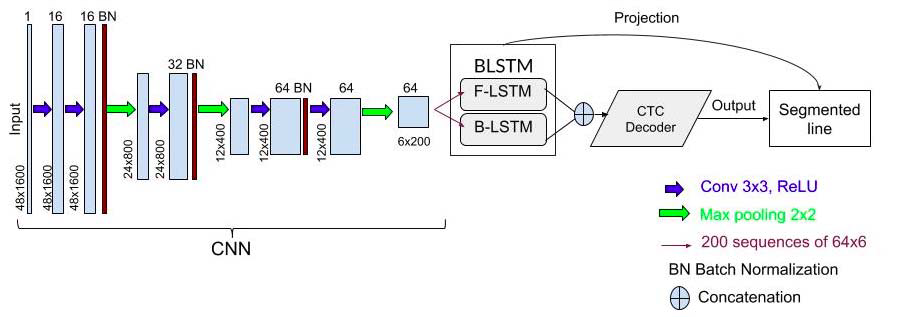
\includegraphics[width=10cm]{images/seg_network.png}
        \caption{Proposed word segmentation network.}
        \label{fig:seg_network}
        \end{figure}
        
        \begin{figure}[!htb]
        \centering
        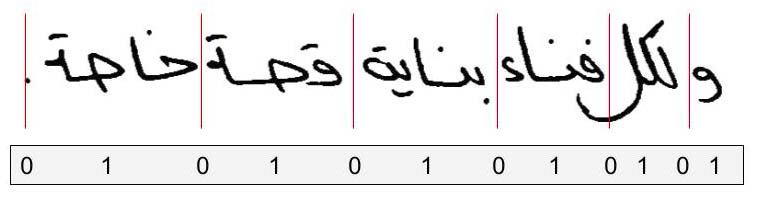
\includegraphics[width=8cm]{images/word_seg.png}
        \caption{Ground truth provided to the CTC (1: word; 0: space).}
        \label{fig:word_seg}
        \end{figure}
    
 \end{itemize}
 
Tested on the standard KHATT Arabic database, the experimental results confirm a segmentation success rate of no less than 96.7\%. \\

This paper \cite{FCN} presents a method for text line segmentation
of challenging historical manuscript images. These manuscript images contain narrow interline spaces with touching components, interpenetrating vowel signs, and inconsistent font types and sizes. In addition, they contain curved, multi-skewed, and multi-directed side note lines Fig \ref{fig:text line problems} within a complex page layout. Therefore, bounding polygon labeling would be very difficult and time consuming. Instead, they rely on line masks that connect the components on the same text line. Then these line masks are predicted using a Fully Convolutional Network (FCN). FCN has been successfully used for text line segmentation of regular handwritten document images. This paper shows that FCN is useful with challenging manuscript images as well. Using a new evaluation metric that is sensitive to over segmentation as well as under segmentation.Test on the new challenging handwritten document dataset. The model achieved 89\% training accuracy and 88\% validation accuracy on average.

\begin{figure}[!htb]
    \centering
    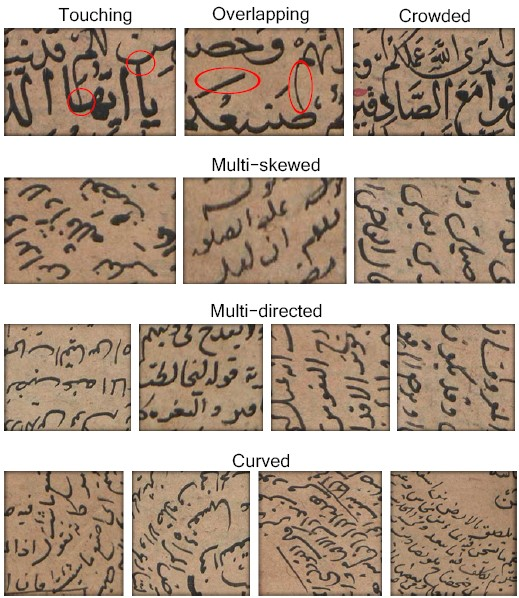
\includegraphics[width=7cm]{images/text line segmentation problems.jpg}
    \caption{Additional text line segmentation problems with challenging handwritten documents. Various writing styles are also noticeable.}
    \label{fig:text line problems}
\end{figure}

\begin{description}
  \item[Their Method] FCN inputs the original images and their pixel level annotations for learning the hypothesis function that can predict whether a pixel belongs to a text line label or not. They used line mask labeling that connects the characters in the same line.
   
  \begin{enumerate}
  \item FCN architecture Fig \ref{fig:fcn_arc}.
  \item Pre-processing Fig \ref{fig:fcn_image}.
  \item Training and testing.
  \item Post-processing Fig \ref{fig:fcn_post}.
  \item Connectivity Component Based Line Extraction Accuracy Metric.
\end{enumerate}
\end{description}


\begin{figure}[!htb]
    \centering
    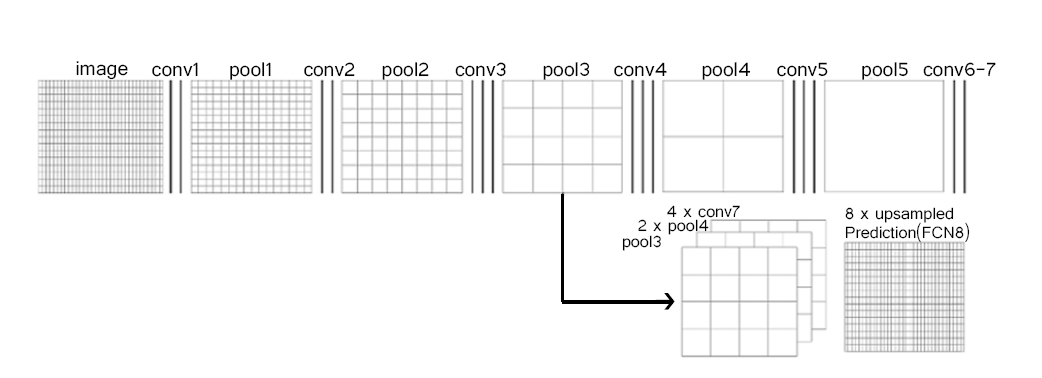
\includegraphics[width=15cm]{images/FCN_arc.png}
    \caption{The FCN architecture. Pooling and prediction layers are shown as grids that show relative coarseness. Convolutional layers are shown as vertical lines. FCN8 4 times upsamples the final layer, 2 times upsamples the pool4 layer and combine them with pool3 layer finally to upsample to the input size.}
    \label{fig:fcn_arc}
\end{figure}

\begin{figure}[!htb]
    \centering
    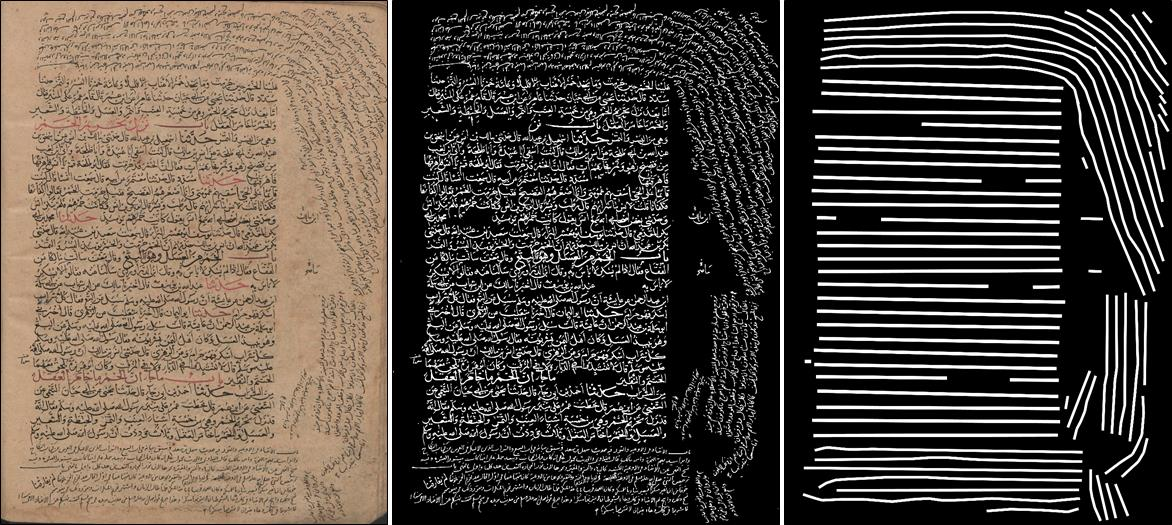
\includegraphics[width=12cm]{images/fcn_image.jpg}
    \caption{A sequence of original, binarized, and labeled document images. Random patches for training are generated from the binarized and labeled images.}
    \label{fig:fcn_image}
\end{figure}
\begin{figure}[!htb]
    \centering
    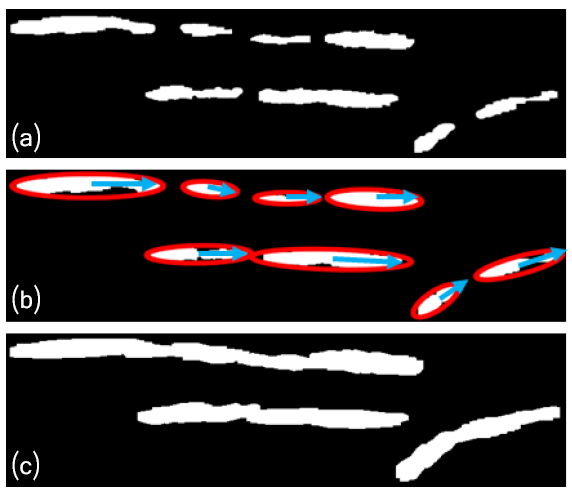
\includegraphics[width=7cm]{images/FCN_post.png}
    \caption{Post processing phases: (a) Predicted line mask may have disconnected components. (b) For each component, an ellipse (red) is fitted and its orientation vector $\theta$ (c) (blue) is computed. (c) Morphological dilation is applied to each component with a narrow kernel in the direction of its fitted ellipse.}
    \label{fig:fcn_post}
\end{figure}

This paper \cite{PP} presented an approach for line and character segmentation based on the PP method. This method was applied to a historical Arabic manuscript collected from the Manuscripts department at Umm Al-Qura University’s Library.
 \begin{figure}[!htb]
    \centering
    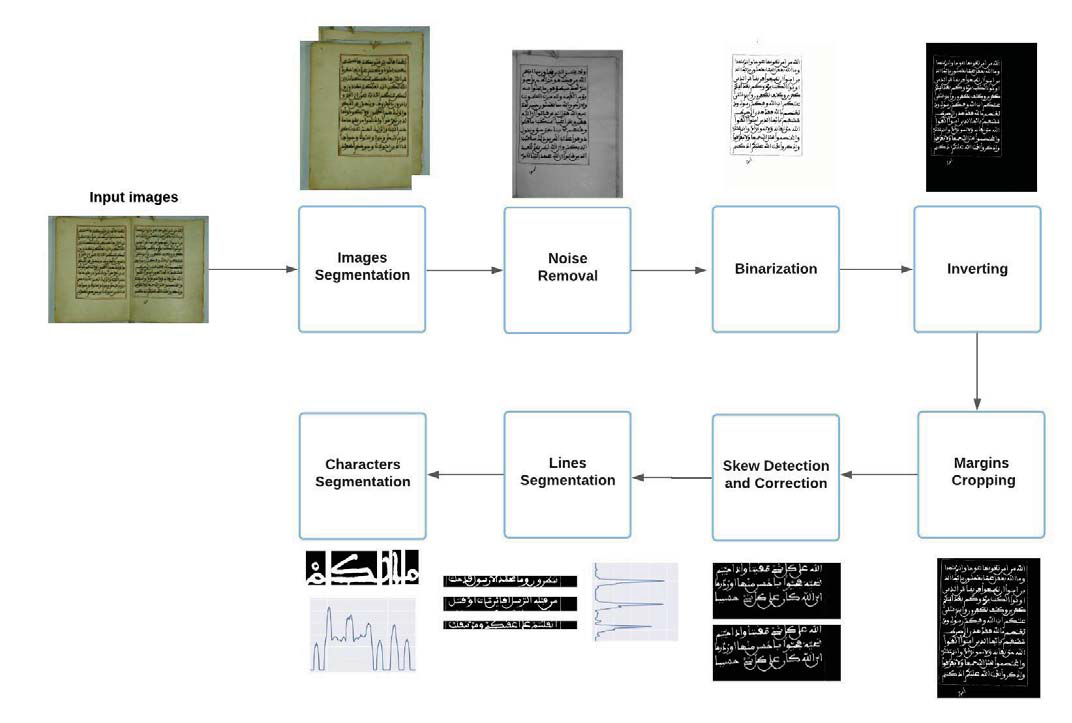
\includegraphics[width=11cm]{images/pp_seg.png}
    \caption{Process of proposed method for line and word segmentation.}
    \label{fig:pp_seg}
\end{figure}
\newline\\
In order to reach excellent segmentation results, it is needed to apply some preprocessing steps to the manuscript such as Images Extraction, Noise Removal, Binarization and Inverting, Margins Cropping, Skew Detection, and Correction then Segmentation. The segmentation step is dividing text images into base components such as lines, words, and characters.
\begin{itemize}[labelindent=1em,labelsep=0.25cm,leftmargin=*]

        \item[\char `A)] \textit{\textbf{Lines Segmentation:}} 
         After the images’ margins have been cropped, images are segmented line by line using the Horizontal PP method, which converts 2D into 1D images by calculating the densities of each row. Then, each line is cropped separately at the lowest density point. Since the manuscript is written in a complex way, the spaces between lines is not totally empty. Therefore, its density from Horizontal PP is not equal to 0. In order to overcome this problem, an opening operation is performed on each image before segmentation. Opening is considered a morphology operation.
        
        \item[\char `B)] \textit{\textbf{Characters Segmentation:}} 
        Another type of segmentation that was performed is character segmentation. In this step, the lines that are obtained from the previous step are divided into separated characters.
        
        This step was applied by using the Vertical PP method. This method works the same way as Horizontal PP in the previous step, except that the direction of calculating the density. in Vertical PP it is calculated on columns instead of rows. The opening operation was also performed on each line before segmentation.
    \end{itemize}

The total number of lines segmented during lines segmentation is 635. The original manuscript contains 657 lines. There were 10 empty segmented lines out of 635. since they contain
parts of the characters from the line above and below them.
Fig. \ref{fig:pp_empty} shows an example of this case. In addition, 15 lines
were overlapped with other lines. Table \ref{table:1} shows the results
summary of lines segmentation.

\begin{figure}[!htb]
    \centering
    
\includegraphics[width=11cm]{images/pp_empty.png}
    \caption{Empty line.}
    \label{fig:pp_empty}
\end{figure}

\begin{table}[!htb]
\centering
\begin{tabular}{|l|l|}
\hline
\textbf{Case}                   & \textbf{Number of Lines} \\ \hline
Total number of segmented lines & 635                      \\ \hline
Correctly segmented             & 610                      \\ \hline
Empty                           & 10                       \\ \hline
Two overlapped                  & 11                       \\ \hline
Three overlapped lines          & 4                        \\ \hline
\end{tabular}
\caption{Lines Segmentation Results Summary.}
\label{table:1}
\end{table}


\section{Word Segmentation}
Word/subword segmentation is an important step in the segmentation phase for segmentation-based Arabic OCR(AOCR) systems since it facilitates working on the character segmentation stage. In addition, it can be employed as a post processing stage after character recognition to increase the recognition rate.\\

In paper \cite{article} 
introduced a segmentation algorithm that uses a technique in which the overlapping Arabic words/sub-words are horizontally separated; they also used a feedback loop between the character segmentation stage and final recognition stage. 

In paper \cite{jawad_h_alkhateeb}
proposed a method for baseline detection and employed it to extract the connected components of each sub-word. After detection of the baseline, an iterative process was used to detect the connected components based on the connected black pixels in the sub-word. \\

\noindent
Arabic writing is cursive; therefore, words and subwords are separated by spaces, so word boundaries are always represented by a space. According  to  this, distances between each pair of consecutive sub-words are obtained. Normally the distances between words are larger than the distances between subwords, thus words can be segmented by comparing this distance against a suitable threshold. This paper is concerned with word segmentation using vertical histogram and connected component analysis. Also, distance  information is very essential in segmenting words. Here, the distances between subwords were measured and compared to an optimal threshold to determine if the distance corresponds to the separation of two words or not. 

\begin{itemize}[labelindent=1em,labelsep=0.25cm,leftmargin=*]
        \item[\char `A)] \textit{\textbf{Baseline Detection:-}} 
        Before  segmenting  the  Arabic  words,  we  need  to detect  the  baseline  as  it  is  believed  that  this  baseline  is  very  essential  in  analyzing  Arabic  text.  Since  the  Arabic  letters  are  usually written along the baseline, hopefully, there should be a peak in the baseline position when we project the written line along the vertical axis of the image.
        The  improved result is shown in Fig. \ref{fig:basline}
 
         \begin{figure}[!htb]
            \centering
            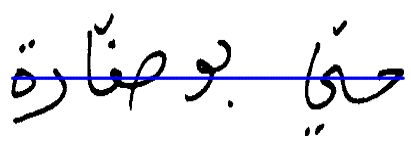
\includegraphics[width=6cm]{images/basline.png}
            \caption{Baseline detection: original result using only vertical projection using both vertical projection and knowledge-support}
            \label{fig:basline}
        \end{figure}
        
        \item[\char `B)] \textit{\textbf{Extracting Connected Components and Sub-Words:-}}  
        
        Segmentation is an essential step that separates the text image objects for the recognition phase. The typical segmentation for the printed binary document is based on the histogram projection analysis and regrouping of the connected components. Arabic writing is cursive  and is such that words are separated by spaces. However,  a  word may contain several sub-words which are a portion  of  the  word including one or more connected letters.
Fig. \ref{fig:subword} shows three Arabic words consisting of one, two, and three sub-words respectively. 

 \begin{figure}[!htb]
    \centering
    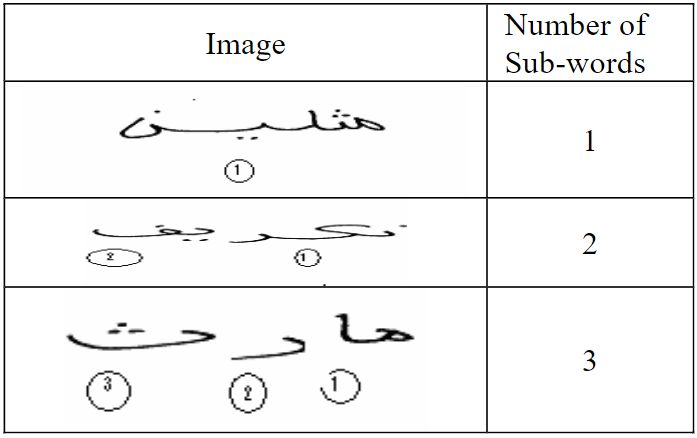
\includegraphics[width=5cm]{images/subword.png}
    \caption{Arabic words with sub-words}
    \label{fig:subword}
\end{figure}

The connected components (CCs) for the line image must be determined.  The  CCs  are  rectangular  boxes  bounding  together  regions of connected objects. The objective of the CCs phase is to  form  rectangles  around  the  connected  object  on  the  image.    The algorithm used to obtain the CCs  are  the  iterative procedure that compares any black pixels in any pair of the line are connected together.    Bounding rectangles are  extended  to  enclose  any  grouping  of  connected  black  pixels.  Fig. \ref{fig:ccs}(a) shows the output of the CCs.  With extracted connect components,    sub-words are segmented  as  follows.  Firstly,  small  parts  like  dots  in  the  image  are  temporally  ignored.  Secondly,  components  whose  coordinates  are  overlapped  on  the x-axis  are  merged  to  obtain  a  combined  large  component,  namely  a sub-word.  Thirdly,  the  distance  of  each  pair  of  consecutive  sub-words  is  obtained,  which will be used to segment words in the next section.
\begin{figure}[!htb]
    \centering
    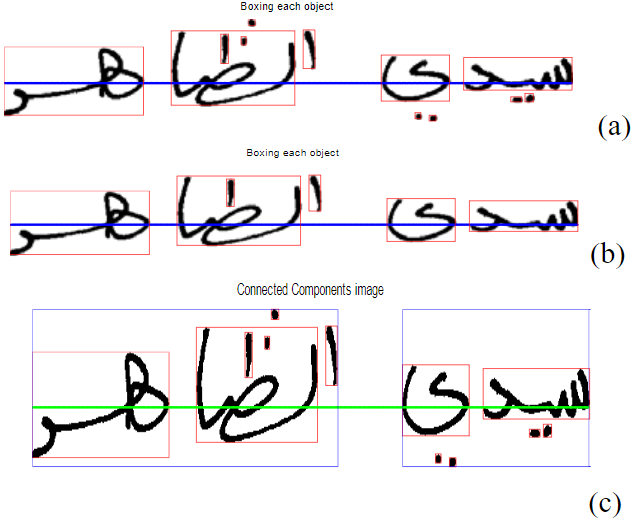
\includegraphics[width=6cm]{images/ccs.png}
    \caption{Examples of extracted connected components (a), sub-words of combined components (b), and detected words (c)}
    \label{fig:ccs}
\end{figure}

\end{itemize}

\noindent
The table \ref{tb:vpp-accuracy-table}shows the testing results of this technique which is tested on 200 images in the test set and the segmentation accuracy is  85%
    

\begin{table}[!htb]
\centering
\begin{tabular}{|l|l|l|l|l|}
\hline
 NO .of Images & Correct Seg. & Under Seg. & Over seg. & Misplaced Seg. \\ \hline
 200  & 85\%  & 90\% & 4\% & 2\% \\ \hline
\end{tabular}
\caption{Results of the accuracy of segmentation}
\label{tb:vpp-accuracy-table}
\end{table}

\section{Word Spotting}
Since, \acrshort{ocr} for manuscript images is impossible, this is due to the semi-cursive nature of Arabic script which is very difficult to explore by algorithms and image processing methods.

\noindent
Word spotting techniques are used to explore and research in the content of Arabic manuscript images. It’s about characterizing segmented handwritten words with a set of points of interest by providing a means of identification and research in these manuscripts. Each word segmented and described by key features will be compared to query words. \\

In \cite{Noureddine} presents a method that facilitates access to the content of images. This method is based on the invariant local detectors and descriptors (scale, rotation, brightness variations) for the detection of this information in the Arabic manuscripts. Word spotting technique allows the matching process between the handwritten words of the query images with the target images. 

The proposed method for the characterization of images of Arabic manuscripts. In the same way, as in the field of the recognition of Latin texts shown in figure \ref{fig:noureddine-word-spotting-}.
\begin{figure}[!htb]
    \centering
    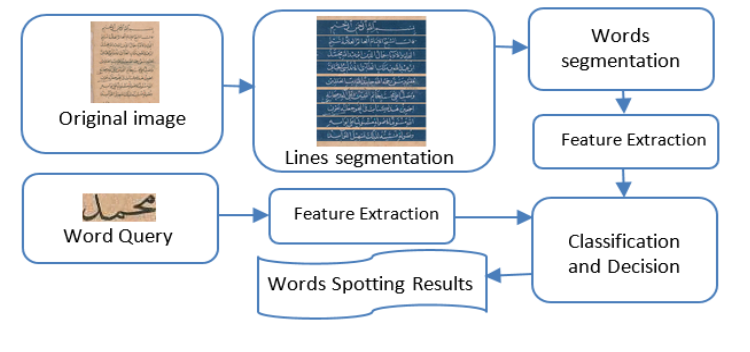
\includegraphics[width=13cm]{images/noureddine-word-spotting.png}
    \caption{Process of the proposed method for word spotting}
    \label{fig:noureddine-word-spotting}
\end{figure}

\begin{itemize}[labelindent=1em,labelsep=0.25cm,leftmargin=*]
        \item[\char `A)] \textit{\textbf{Acquisition and Pre-processing:-}} \\
        They collect manually huge scanned manuscripts, then a  series of pre-processing can be applied to images such as Contrast Enhancement, straightening, curvature correction, detail emphasis, and spreading of levels. This processing can improve the quality of the images and also their segmentation. An example of the collected data after preprocessing shown in the figure \ref{fig:noureddine-data}
        \begin{figure}[!htb]
            \centering
            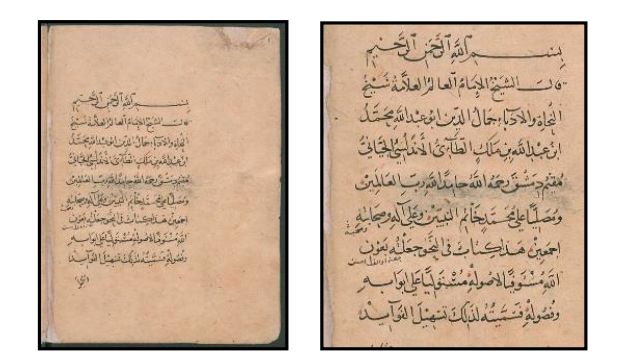
\includegraphics[width=10cm]{images/noureddine-data.png}
            \caption{Example of the scanned image left and right after pre-processing}
            \label{fig:noureddine-data}
        \end{figure}
        
        \item[\char `B)] \textit{\textbf{Lines Segmentation:-}} \\
        Line segmentation is necessary to locate the position of words for the word spotting method. The line was extracted using grayscale images to facilitate line detection despite some overlaps. They used the projection algorithm in \cite{ManmathaProjectionAlgorithm}. The projection function $f(y)$ that has applied for a gray level image of intensity $I(x, y)$ is as follows:
        \begin{equation}
            f(y) = \sum_{x=0}^w I(x, y)
        \end{equation}
        
        The project profile $f(y)$ of the image $I$ for the line x is illustrated in Fig \ref{fig:noureddine-word-line}. Additional high-frequency noise may affect this function. In this case, it is necessary to smooth this signal with the aid of a filter, we can perform a convolution with a Gaussian filter in the equation \ref{equ:gaussian-filter} in order to eliminate the high-frequency noise in the signal of the function in the equation \ref{equ:signal-function}
        
        \begin{equation}
            p(y) = f(y)*g(y,\sigma) 
        \label{equ:gaussian-filter}
        \end{equation}
        
        \begin{equation}
            g(y, \sigma) = \frac{1}{\sigma \sqrt{2 \pi}} e^{-\frac{y^2}{2\sigma^2}}
        \label{equ:signal-function}
        \end{equation}
        
        \item[\char `C)] \textit{\textbf{Word Segmentation:-}} \\
        In order to extract all the information in each word to facilitate the task to the processing algorithms. Some image preprocessing techniques like applying binary images for the extraction of the related components, then morphological dilation of the binary images allows the fusion of the isolated characters and the pseudo-words. The projection at each line provides the words. The main problem with this technique is its sensitivity to overlapping words. Detection of the related components at the level of each line in the binary images to also locate the words.
        The following figure \ref{fig:noureddine-word-line} shows an example of segmentation of elements (isolated characters, pseudo words, and words).
        
        \begin{figure}[!htb]
            \centering
            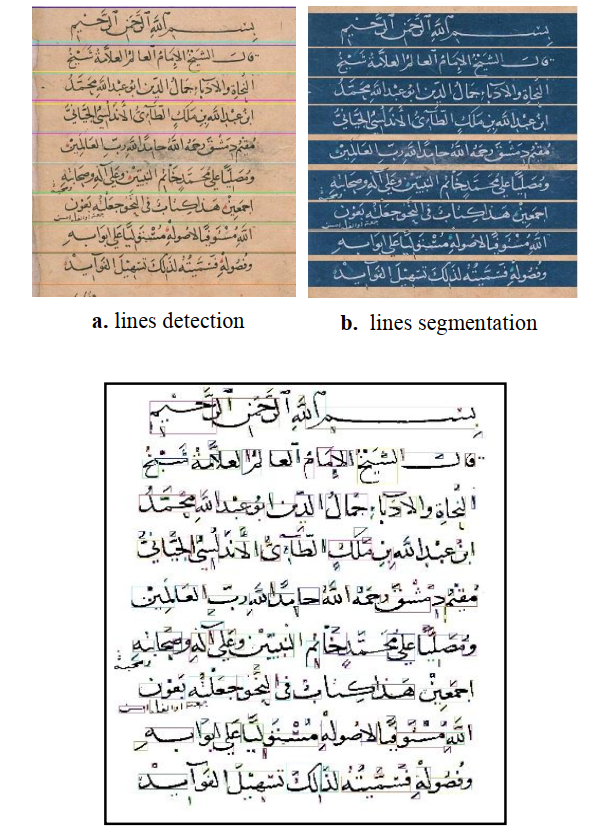
\includegraphics[width=8cm]{images/noureddine-line-word-segmentation.png}
            \caption{Segmentation results}
            \label{fig:noureddine-word-line}
        \end{figure}
        
        \item[\char `D)] \textit{\textbf{Feature Extraction:-}} \\
        As part of the Word Spotting method of detecting words at the level of Arabic handwriting, all types of manuscripts must be considered. However, some documents, such as manuscripts with different colors but with identical intensities, require the use of color to ensure correct key points extraction. The second possible variation concerns the relationship between the reliability and the algorithmic cost of the detector. Indeed, the SIFT detector extracts robust and fewer points but at the cost of additional calculations. In this case, the use of SURF detectors to extract feature elements (isolated characters, pseudo words, or words) can be effective and is faster compared to other detectors
        
        \item[\char `E)] \textit{\textbf{Classification, Matching and Decision:-}} \\
        By using SURF interest points. The comparison between two interest points can be done with several methods. Choice of such a method can be made per processing costs. Interest points are characterized by their properties. The comparison can therefore be carried out in two stages: The first step of comparison between two points is carried out by examining the signs of traces of the Hessian matrix. The sign of the trace of the Hessian matrix thus represents the sign of the Laplacian and the meaning of blobs. The second step of the comparison consists in calculating the distance between the descriptor vectors of the two interest points. The most commonly used comparison methods are based on correlation and on the calculation of vector distances. The distance between two vectors v and u of the two descriptors of interest points can be calculated with the Euclidean distance or with the Mahalanobis distance.
        \item[\char `F)] \textit{\textbf{Results and application GUI:-}} \\
        The results of matching with the Word Spotting method give many occurrences of the name "Mohamed \<محمد>" equal to twice shown in figure \ref{fig:noureddine-word-spotting-results}. We used three types of query images (color, grayscale and binary) and we got the same result. Therefore, this method can be applied to a set of images of the same manuscript, which makes it possible to search all the occurrences of the query word

        \begin{figure}[!htb]
            \centering
            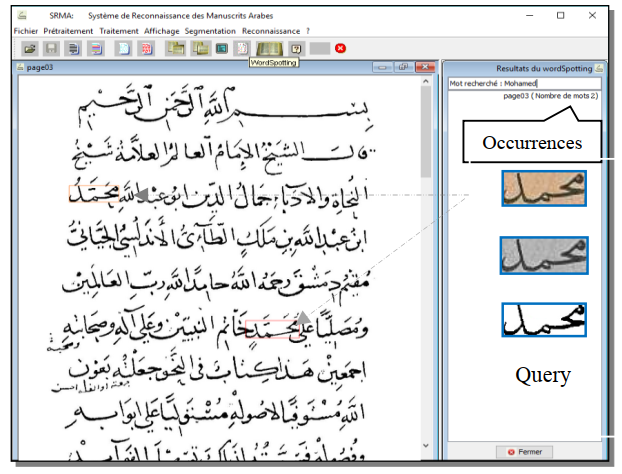
\includegraphics[width=12cm]{images/noureddine-word-spotting-application.png}
            \caption{Word spotting results}
            \label{fig:noureddine-word-spotting-results}
        \end{figure}

\end{itemize}


\section{Implementation Approach}
After reviewing different papers addressing the problem of digitizing historical Arabic manuscripts documents, as previously mentioned, that \acrshort{htr} systems are inefficient for recognizing the historical handwritten documents, so we decided to follow the approach of the pattern recognition technique to build an intelligent system able to understand handwritten manuscript documents by matching the pattern with manually collected huge labeled data of segmented words. 
Since the goal of this system is to digitize the image manuscripts, then word spotting will not be enough for that purpose as the aim of word spotting is to final all the instances of a query word in a dataset of images. We need also a word recognition technique to recognize the content of the word image. So we will use a special text-embedded technique to extract textual features to produce a common representation that enables the machine to recognize and extract it when having a particular image feature. \acrfull{phoc} is a new method to achieve this scenario which encodes if a particular character appears in a particular spatial region of the string \cite{WORDSPOTTING}. We will use this method with a modified version. \\


We have decided to go through VML-HD dataset \cite{VMLHD}, as it has a lot of images for different Arabic manuscripts and different fonts with different styling word shapes, we will do data cleaning to remove mislabeled data and to prepare it for word spotting techniques. In addition, we will augment the data using morphology techniques for image preprocessing that's because it's unbalanced and has low correlations with the number of collected words. \\

In word and line segmentation, we want to segment the line first, so we will use morphology operations after doing some preprocessing like normalization, binarization, median filtering logic,  dilation, and erosion for edge detection improvement, then we finally extract the contours from dilation operation as segmented lines. In word segmentation, we will use morphological operation techniques to extract each word of the line as cropped image \cite{PP}.